\documentclass[aspectratio=169,handout]{beamer}
%\documentclass[aspectratio=169,handout]{beamer}
\usepackage[utf8]{inputenx} % For æ, ø, å
\usepackage{csquotes}       % Quotation marks
\usepackage{microtype}      % Improved typography
\usepackage{amssymb}        % Mathematical symbols
\usepackage{mathtools}      % Mathematical symbols
\usepackage[absolute, overlay]{textpos} % Arbitrary placement
\setlength{\TPHorizModule}{\paperwidth} % Textpos units
\setlength{\TPVertModule}{\paperheight} % Textpos units
\usepackage{tikz}
\usetikzlibrary{overlay-beamer-styles}  % Overlay effects for TikZ


\AtBeginSection{\frame{\sectionpage}}
\AtBeginSubsection{\frame{\subsectionpage}}

\usepackage{hyperref}
\usepackage{svg}
%\usefonttheme{serif}

\usepackage{xfrac}
\usepackage{soul} % Colored text and highlighting, respectively
\usepackage{xcolor}
\usepackage{tikz-cd} % For commutative diagrams
\usepackage{tikz-3dplot}
\usetikzlibrary{angles}
\RequirePackage{pgfplots}
\usepackage{mathtools}
\usepackage{answers}
\usepackage{setspace}
\usepackage{graphicx}
\usepackage{enumerate}
\usepackage{multicol}
%\usepackage{mathrsfs}
\usepackage{amsmath}
\usepackage{marvosym,wasysym} %fucking smileys
\usepackage{float}
\usepackage{morefloats}
\usepackage{pgf,tikz}
\pgfplotsset{compat=1.15}
%\usepackage{mathrsfs}
\usetikzlibrary{arrows}
\usepackage{subcaption}
\usepackage[most]{tcolorbox}
%\tcbuselibrary{theorems}


\usepackage{fancyvrb}
\usepackage{longtable,booktabs}
\usepackage{stackrel}
\usepackage{animate}
\usepackage[percent]{overpic}
\usepackage{stmaryrd}
\definecolor{lighter_csu_green}{RGB}{60,133,77}
\definecolor{darker_csu_green}{RGB}{30,77,43}
\definecolor{csu_gold}{RGB}{198,184,77}
\definecolor{gray}{RGB}{150,150,150}
\definecolor{dim_csu_gold}{RGB}{178,164,57}
\newcommand\boldgreen[1]{\textcolor{lighter_csu_green}{\emph{\textbf{#1}}}}
\newcommand\boldgold[1]{\textcolor{csu_gold}{\textbf{#1}}}
\newcommand\bolddimgold[1]{\textcolor{dim_csu_gold}{\textbf{#1}}}
\newcommand\grey[1]{\textcolor{gray}{#1}}

\newtcbtheorem{thm}{Theorem}{%
  breakable,
  colback=black,
  colframe=dim_csu_gold,
  fonttitle=\bfseries,
  coltitle=darker_csu_green,
  coltext=white
}{thm}
%
\newtcbtheorem{lemm}{Lemma}{%
  breakable,
  colback=black,
  colframe=dim_csu_gold,
  fonttitle=\bfseries,
  coltitle=darker_csu_green,
  coltext=white
}{lem}

\newtcbtheorem{proposition}{Proposition}{%
  breakable,
  colback=black,
  colframe=dim_csu_gold,
  fonttitle=\bfseries,
  coltitle=darker_csu_green,
  coltext=white
}{prop}




%\usepackage{MnSymbol}
%border matrix
\makeatletter
\newif\if@borderstar
\def\bordermatrix{\@ifnextchar*{%
\@borderstartrue\@bordermatrix@i}{\@borderstarfalse\@bordermatrix@i*}%
}
\def\@bordermatrix@i*{\@ifnextchar[{\@bordermatrix@ii}{\@bordermatrix@ii[()]}}
\def\@bordermatrix@ii[#1]#2{%
\begingroup
\m@th\@tempdima8.75\p@\setbox\z@\vbox{%
\def\cr{\crcr\noalign{\kern 2\p@\global\let\cr\endline }}%
\ialign {$##$\hfil\kern 2\p@\kern\@tempdima & \thinspace %
\hfil $##$\hfil && \quad\hfil $##$\hfil\crcr\omit\strut %
\hfil\crcr\noalign{\kern -\baselineskip}#2\crcr\omit %
\strut\cr}}%
\setbox\tw@\vbox{\unvcopy\z@\global\setbox\@ne\lastbox}%
\setbox\tw@\hbox{\unhbox\@ne\unskip\global\setbox\@ne\lastbox}%
\setbox\tw@\hbox{%
$\kern\wd\@ne\kern -\@tempdima\left\@firstoftwo#1%
\if@borderstar\kern2pt\else\kern -\wd\@ne\fi%
\global\setbox\@ne\vbox{\box\@ne\if@borderstar\else\kern 2\p@\fi}%
\vcenter{\if@borderstar\else\kern -\ht\@ne\fi%
\unvbox\z@\kern-\if@borderstar2\fi\baselineskip}%
\if@borderstar\kern-2\@tempdima\kern2\p@\else\,\fi\right\@secondoftwo#1 $%
}\null \;\vbox{\kern\ht\@ne\box\tw@}%
\endgroup
}
\makeatother

\usetheme{UiB}

%For easier reading
\setbeamersize{text margin left=40pt,text margin right=40pt}
\renewcommand{\baselinestretch}{1.3}


%% FONT STUFF
\usefonttheme[onlymath]{serif}

%Commands
\makeatletter
\DeclareFontFamily{OMX}{MnSymbolE}{}
\DeclareSymbolFont{MnLargeSymbols}{OMX}{MnSymbolE}{m}{n}
\SetSymbolFont{MnLargeSymbols}{bold}{OMX}{MnSymbolE}{b}{n}
\DeclareFontShape{OMX}{MnSymbolE}{m}{n}{
    <-6>  MnSymbolE5
   <6-7>  MnSymbolE6
   <7-8>  MnSymbolE7
   <8-9>  MnSymbolE8
   <9-10> MnSymbolE9
  <10-12> MnSymbolE10
  <12->   MnSymbolE12
}{}
\DeclareFontShape{OMX}{MnSymbolE}{b}{n}{
    <-6>  MnSymbolE-Bold5
   <6-7>  MnSymbolE-Bold6
   <7-8>  MnSymbolE-Bold7
   <8-9>  MnSymbolE-Bold8
   <9-10> MnSymbolE-Bold9
  <10-12> MnSymbolE-Bold10
  <12->   MnSymbolE-Bold12
}{}

\let\llangle\@undefined
\let\rrangle\@undefined
\DeclareMathDelimiter{\llangle}{\mathopen}%
                     {MnLargeSymbols}{'164}{MnLargeSymbols}{'164}
\DeclareMathDelimiter{\rrangle}{\mathclose}%
                     {MnLargeSymbols}{'171}{MnLargeSymbols}{'171}
\makeatother
\newcommand{\directedintproduct}[2]{\llparenthesis \hspace*{.5mm}#1 , #2\hspace*{.5mm} \rrparenthesis}
\newcommand{\multivecinnerproduct}[2]{\llangle \hspace*{.5mm} #1, #2 \hspace*{.5mm} \rrangle}
\newcommand{\trace}{\mathrm{tr}}
\newcommand{\tangentpart}{\boldsymbol{t}}
\newcommand{\normalpart}{\boldsymbol{n}}
\newcommand{\R}{\mathbb{R}}
\newcommand{\C}{\mathbb{C}}
\newcommand{\opens}{\mathcal{O}}
\newcommand{\hilbert}{\mathcal{H}}
\newcommand{\algebra}{\mathcal{A}}
\newcommand{\ideals}{\mathcal{I}}
\newcommand{\functionals}{\mathcal{M}}
\newcommand{\spec}{\mathrm{spec}}
\newcommand{\clifford}{\mathrm{C}\ell}
    \newcommand\quotient[2]{
        \mathchoice
            {% \displaystyle
                \text{\raise1ex\hbox{$#1$}\Big/\lower1ex\hbox{$#2$}}%
            }
            {% \textstyle
                #1\,/\,#2
            }
            {% \scriptstyle
                #1\,/\,#2
            }
            {% \scriptscriptstyle
                #1\,/\,#2
            }
    }

% Special Commands
\newcommand{\bigslant}[2]{{\raisebox{.2em}{$#1$}\left/\raisebox{-.2em}{$#2$}\right.}}
\newcommand{\RE}{\mathrm{Re}}
\newcommand{\IM}{\mathrm{Im}}
\newcommand{\multivectorbundle}{\mathcal{G}(M,g)}
\newcommand{\multivectorfields}{\mathcal{G}(M)}
\newcommand{\differentialforms}{\mathcal{G}^*(M)}
\newcommand{\kvectorfields}[1]{\mathcal{G}^{#1}(M)}
\newcommand{\evenfields}{\mathcal{G}^{[0]}(M)}
\newcommand{\oddfields}{\mathcal{G}^{[1]}(M)}
\newcommand{\id}{\mathrm{id}}
\newcommand{\innerproduct}[2]{\left\langle #1, #2 \right\rangle_{L_2(\Sigma)}}
%\newcommand{\algebra}[1]{\mathcal{A}_{#1}}
\newcommand{\grad}{\boldsymbol{\nabla}}
\newcommand{\dirac}{\boldsymbol{D}}
\newcommand{\geometricalg}{\mathcal{G}(V)}
\newcommand{\spacealg}{\mathcal{G}_3}
\newcommand{\dual}[1]{\overset{$\star$}&{#1}}
\newcommand{\G}{\mathcal{G}}
\newcommand{\cauchy}{\mathcal{C}}
\newcommand{\poisson}{\mathcal{P}}
\newcommand{\tangent}{\boldsymbol{t}}

\newcommand{\openO}{\mathcal{O}}
\newcommand{\openU}{\mathcal{U}}
\newcommand{\characters}{\mathfrak{M}}
\newcommand{\Span}{\operatorname{Span}}
\newcommand{\paravectors}{\mathcal{P}}
\newcommand{\paravectorfields}{\mathcal{P}(M)}
\newcommand{\monogenics}{\mathcal{M}}
\newcommand{\dualmonogenics}{\mathcal{M}^*}
\newcommand{\Grassmannian}[2]{\textrm{Gr}(#1,#2)}
\newcommand{\spinalgebra}{\mathfrak{spin}(n)}
\newcommand{\spingroup}{\operatorname{Spin}(n)}
\newcommand{\ball}{\mathbb{B}}
\newcommand{\disk}{\mathbb{D}}
\newcommand{\projection}{\operatorname{P}}
\newcommand{\vectorspace}{\mathbb{V}}
\newcommand{\multivectorfieldson}[1]{\mathcal{G}(#1)}
\newcommand{\biparavectorfieldson}[1]{\mathcal{G}_n(#1)^{0+2}}
\newcommand{\spinnorm}[1]{\|#1\|_{L_2}}
\newcommand{\rejection}{\operatorname{R}}
\newcommand{\vectorpotential}{\mathbf{A}}
\newcommand{\current}{\blade{j}}
\newcommand{\magneticbivector}{\blade{b}}
\newcommand{\cross}{\boldsymbol{\times}}
\newcommand{\blade}[1]{\boldsymbol{#1}}
\newcommand{\intcurrent}[1]{\left[ #1 \right]}
\newcommand{\spacetime}{\boldsymbol{\gamma}}
\newcommand{\gradst}{\boldsymbol{\nabla}_{\textrm{ST}}}
\newcommand{\boundary}{{\partial M}}
\newcommand{\normalcurrent}{\blade{j}^{\blade{\nu}}}
\newcommand{\tangentialcurrent}{\blade{j}^{\blade{I}_\partial}}
\newcommand{\normal}{\blade{\nu}}
\newcommand{\pseudoscalar}{\blade{I}}

\newcommand{\kforminnerproduct}[2]{\llangle #1, #2 \rrangle}
\newcommand{\contract}{\hspace*{.5mm} \lrcorner \hspace*{.5mm}}

\DeclarePairedDelimiter\angles{\langle}{\rangle}
\newcommand{\proj}[2]{\angles*{#2}_{#1}}

% Forms stuff
\newcommand{\harmonicfields}[1]{\mathcal{H}^{#1}(M)}
\newcommand{\monogenicex}[1]{\mathcal{M}^{#1}_{\textrm{ex}}(M)}
\newcommand{\monogenicco}[1]{\mathcal{M}^{#1}_{\textrm{co}}(M)}
\newcommand{\monogenicdirichlet}[1]{\mathcal{M}^{#1}_D(M)}
\newcommand{\monogenicneumann}[1]{\mathcal{M}^{#1}_N(M)}
\newcommand{\exactfields}[1]{\mathcal{E}^{#1}(M)}
\newcommand{\coexactfields}[1]{\mathcal{C}^{#1}(M)}
\newcommand{\monogenicfields}[1]{\mathcal{M}^{#1}(M)}
\newcommand{\cliffordoplus}{\stackrel{C\ell}{\oplus}}
\newcommand{\bivector}{\blade{B}}
\newcommand{\smoothfields}{\mathfrak{X}}

\definecolor{light-gray}{gray}{0.30}
\makeatletter
\def\mathcolor#1#{\@mathcolor{#1}}
\def\@mathcolor#1#2#3{%
  \protect\leavevmode
  \begingroup
    \color#1{#2}#3%
  \endgroup
}
\makeatother
%\newcommand{\blank}{\raisebox{-.3ex}{\mathcolor{light-gray}{\text{\LARGE$\bullet$}}}}
\newcommand{\blank}{\raisebox{-.3ex}{\mathcolor{light-gray}{\text{\large$\blacksquare$}}}}

\author{Colin Roberts}
\setbeamercolor{title}{fg=white}
\title{Hodge Theory, Gelfand Theory, and Clifford Analysis Applied to Tomography}
\setbeamercolor{subtitle}{fg=white}
\subtitle{}

\setcounter{tocdepth}{1}


\begin{document}
\setbeamercolor{background canvas}{bg=black}
\setbeamercolor{normal text}{fg=white}
\setbeamercolor{itemize/enumerate body}{fg=white}
\setbeamercolor{itemize/enumerate subbody}{fg=white}
\setbeamercolor{itemize/enumerate subsubbody}{fg=white}
\setbeamercolor{section in toc}{fg=white}
\setbeamercolor{subsection in toc}{fg=white}
\setbeamercolor{section name}{fg=white}
\setbeamercolor{subsection name}{fg=white}
\color{white}

\begin{frame}{Overview}
\tableofcontents
\end{frame}

\section{Introduction}

\begin{frame}{Motivating problems}
\vfill
\begin{itemize}
\pause
\item \boldgreen{Electrical Impedance Tomography (EIT)} asks whether one can determine the conductivity of a medium from the voltage-to-current map.
\pause
\item The \boldgreen{Calder\'on problem} replaces the medium with a manifold $M$, conductivity with $g$, and replaces the voltage-to-current map with the Dirichlet-to-Neumann operator $\Lambda$.
\end{itemize}
\vfill
\end{frame}

\begin{frame}{Other questions}
\vfill
    \begin{itemize}
        \pause
        \item What topological information can we retrieve from functions on a manifold?

        \pause
        \item Do these functions also contain metric data?

        \pause
        \item Can we access these functions from the boundary?
    \end{itemize}
\vfill
\end{frame}

\subsection{Preliminaries}

\begin{frame}{Clifford and geometric algebras}
\vfill
\pause
Let $V$ be a vector space over a field $K$ with symmetric bilinear form $g$.
\begin{itemize}
        \pause
        \item Define the tensor algebra
        \[
        \mathcal{T}(V) \coloneqq \bigoplus_{j=0}^\infty V^{\otimes_j} = K \oplus (V \otimes V) \oplus (V \otimes V \otimes V) \oplus \cdots.
        \]
        \pause
        \item The associated \boldgreen{Clifford algebra} is the quotient
        \[
        C\ell(V,g) \coloneqq \mathcal{T}(V)/ \langle \blade{v} \otimes \blade{v} - g(\blade{v},\blade{v})\rangle.
        \]
\end{itemize}
\vfill
\end{frame}

\begin{frame}{Geometric and exterior algebras}
\vfill
\begin{itemize}
        \pause
        \item If $g$ is non-degenerate then we have a \boldgreen{geometric algebra}
        \[
        \G \coloneqq C\ell(V,g).
        \]
        \pause
        \item The completely degenerate case is the \boldgreen{exterior algebra}
        \[
        \bigwedge(V) \coloneqq C\ell(V,0).
        \]
\end{itemize}
\vfill
\end{frame}

\begin{frame}{Algebraic structure}
\vfill
\pause
$\G$ is generated by scalars and vectors given how $\otimes$ acts in the quotient.
\begin{itemize}
    \pause
    \item Given vectors $\blade{u}, \blade{v} \in \G$ we can take the product
    \[
    \blade{u}\blade{v} = \underbrace{\blade{u}\cdot \blade{v}}_{\textrm{scalar}} + \underbrace{\blade{u}\wedge \blade{v}}_{\textrm{bivector}}.
    \]
\begin{itemize}
    \pause
    \item The scalar part is symmetric: $\blade{u}\cdot \blade{v} = g(\blade{u},\blade{v})$.
    \pause
    \item The bivector part is antisymmetric: $\blade{u}\wedge \blade{v} = -\blade{v}\wedge \blade{u}$.
\end{itemize}
\end{itemize}
\vfill
\end{frame}

\begin{frame}{Multivectors}
\vfill
\begin{itemize}
    \pause
        \item $\G$ is graded and of dimension $2^n$.
    \begin{itemize}
        \pause
        \item Grade-$r$ elements, $\G^r$, called \boldgreen{$r$-vectors}.
        \pause
        \item $\proj{r}{A}\in \G^r$ extracts the grade-$r$ part of an arbitrary element $A$.
        \pause
        \item There are ${n \choose r}$ independent \boldgreen{$r$-blades} of the form $\blade{A_r}=\blade{v}_1 \wedge \cdots \wedge\blade{v}_r$.
        \pause
        \item Elements of the even grade subalgebra, $\G^+$, are called \boldgreen{spinors}.
    \end{itemize}
        \pause
        \item Since $\displaystyle{\G=\bigoplus_{r=0}^n \G^r}$ a general \boldgreen{multivector} is $\displaystyle{A = \sum_{r=0}^n \proj{r}{A}}$.
\end{itemize}

\begin{figure}[H]
    \centering
    \def\svgwidth{\columnwidth}
\resizebox{\textwidth}{!}{\input{figures/wedge_product.pdf_tex}}
\end{figure}
\vfill
\end{frame}

\begin{frame}{Algebraic Structure}
\vfill
\begin{itemize}
\pause
\item Extend the multiplication from vectors to multivectors.
\pause
\item On homogeneous elements,
\[
A_r B_s = \proj{|r-s|}{A_r B_s} + \proj{|r-s|+2}{A_r B_s} + \cdots + \proj{r+s}{A_r B_s}
\]
\pause
\item The most important products for us are
\begin{align*}
A_r \wedge B_s &\coloneqq \proj{r+s}{A_r B_s}\\
{A_r} \contract B_s &\coloneqq \proj{s-r}{A_r B_s}
\end{align*}
\end{itemize}
\vfill
\end{frame}

\begin{frame}{Reciprocals and reverses}
\vfill
\begin{itemize}
\pause
\item Given any vector basis $\blade{e}_i$, define the \boldgreen{reciprocal vectors} by $\blade{e}^i\cdot \blade{e}_j = \delta^i_j$.
\pause
\item The \boldgreen{reverse} $\dagger$ is extended linearly from the action on $r$-blades
\[
\blade{A_r}^\dagger = (\blade{v}_1 \wedge \cdots \wedge\blade{v}_r)^\dagger = \blade{v}_r \wedge \cdots \wedge\blade{v}_1.
\]
\end{itemize}
\vfill
\end{frame}


\begin{frame}{Inner product and norm}
\vfill
\begin{itemize}
\pause
\item Define the \boldgreen{multivector inner product} and \boldgreen{multivector norm} by
\[
A \ast B \coloneqq \proj{}{A^\dagger B} \eqqcolon |A|^2
\]
\pause
\item Reverse $\dagger$ is the adjoint operator
\begin{align*}
(CA) \ast B &= A \ast (C^\dagger B)\\
(AC) \ast B &= A \ast (BC^\dagger).
\end{align*}
\pause
\item \boldgold{$g$ definite $\implies$ $\ast$ and $|\blank|$ definite.}
\end{itemize}
\vfill
\end{frame}

\begin{frame}{Blades and subspaces}
\vfill
\begin{itemize}
\pause
\item If $|\blade{U_r}|=\pm 1$, then $\blade{U_r}$ is a \boldgreen{unit blade}.
\pause
\item Unit $r$-blades correspond to subspaces $U\subset V$ (points in $\Grassmannian{r}{n}$).
\pause
\item The \boldgreen{projection} of $A$ into a subspace $\blade{U_r}$ by
\[
\projection_{\blade{U_r}} (A) \coloneqq A\contract \blade{U_r}\blade{U_r}^{-1}.
\]
\end{itemize}
\vfill
\end{frame}

\begin{frame}{Pseudoscalars}
\vfill
\begin{itemize}
\pause
\item \boldgreen{Pseudoscalars} are the grade-$n$ elements.
\pause
\item For example, the volume element
\[
\blade{\mu} = \blade{e}_1 \wedge \cdots \wedge \blade{e}_n.
\]
\pause
\item We define the \boldgreen{unit pseudoscalar} (which corresponds to $V\subset V$) by
\[
\pseudoscalar \coloneqq \frac{1}{|\blade{\mu}|} \blade{\mu}.
\]
\end{itemize}
\vfill
\end{frame}

\begin{frame}{Duality}
\vfill
\begin{itemize}
\pause
\item The \boldgreen{dual} $\perp$ of a multivector $A$ is
\[
A^\perp \coloneqq A \pseudoscalar^{-1} \in \G^{n-r}.
\]
\pause
\item The \boldgreen{Hodge star} $\star_g$ of a multivector $A$ is
\[
\star_g A = (\pseudoscalar^{-1}A)^\dagger.
\]
\pause
\item Dual exchanges products $(A \contract B)^\perp = A \wedge B^\perp$.
\end{itemize}
\vfill
\end{frame}

\begin{frame}{Examples}
\vfill
\begin{itemize}
\pause
\item Define $\G_{p,q}$ by $\blade{e}_i^2=-1$ for $i=1,\dots,p$ and $\blade{e}_i^2=+1$ otherwise.
\pause
\item $\G_{1,3}$ is the \boldgreen{spacetime algebra}.
\pause
\item $\G_{1,3}^2 \cong \mathfrak{spin}(1,3)$ which is the Lie algebra of the Lorentz group.
\pause
\item \boldgreen{Quaternion algebra $\mathbb{H}$} is isomorphic to $\G_{0,3}^+$.
\pause
\item \boldgreen{Complex algebra $\C$} is isomorphic to $\G_{0,2}^+$.
\begin{itemize}
\pause
\item Standard basis $\blade{e}_1,\blade{e}_2$, and $\blade{e}_{12}\coloneqq \blade{e}_1\blade{e}_2$. Then $\blade{e}_{12}^2 = -1$.
\pause
\item Right multiplication of vectors by $\blade{e}_{12}$ rotates counter-clockwise by $\pi/2$.
\end{itemize}
\end{itemize}
\vfill
\end{frame}

\section{Clifford analysis}

\begin{frame}{Multivector Fields}
\vfill
\begin{itemize}
\pause
\item $(M,g)$ is a smooth, compact, connected, oriented $n$-dimensional Riemannian manifold.
\pause
\item \noindent\boldgold{{\underline{Idea:}} Form the Clifford algebras on tangent spaces.}
    \begin{itemize}
        \pause
        \item Form the \boldgreen{geometric algebra bundle}
        \[
        \G M \coloneqq \bigsqcup_{p\in M} C\ell(T_pM,g_p).
        \]
        \pause
        \item The \boldgreen{(smooth) multivector fields $\smoothfields(M)$} are the sections of $\G M$.
    \end{itemize}
    \pause
    \item Take same naming scheme and notation: $\smoothfields^r(M)$, $\smoothfields^+(M)$, etc.
\end{itemize}
\vfill
\end{frame}

\begin{frame}{The $z$-variables}
define those here and then give an example which I plot
\end{frame}

\begin{frame}{Scalar field}
\vfill
The scalar field $A_0 = \proj{}{something}$
\begin{figure}[h]
         \centering
         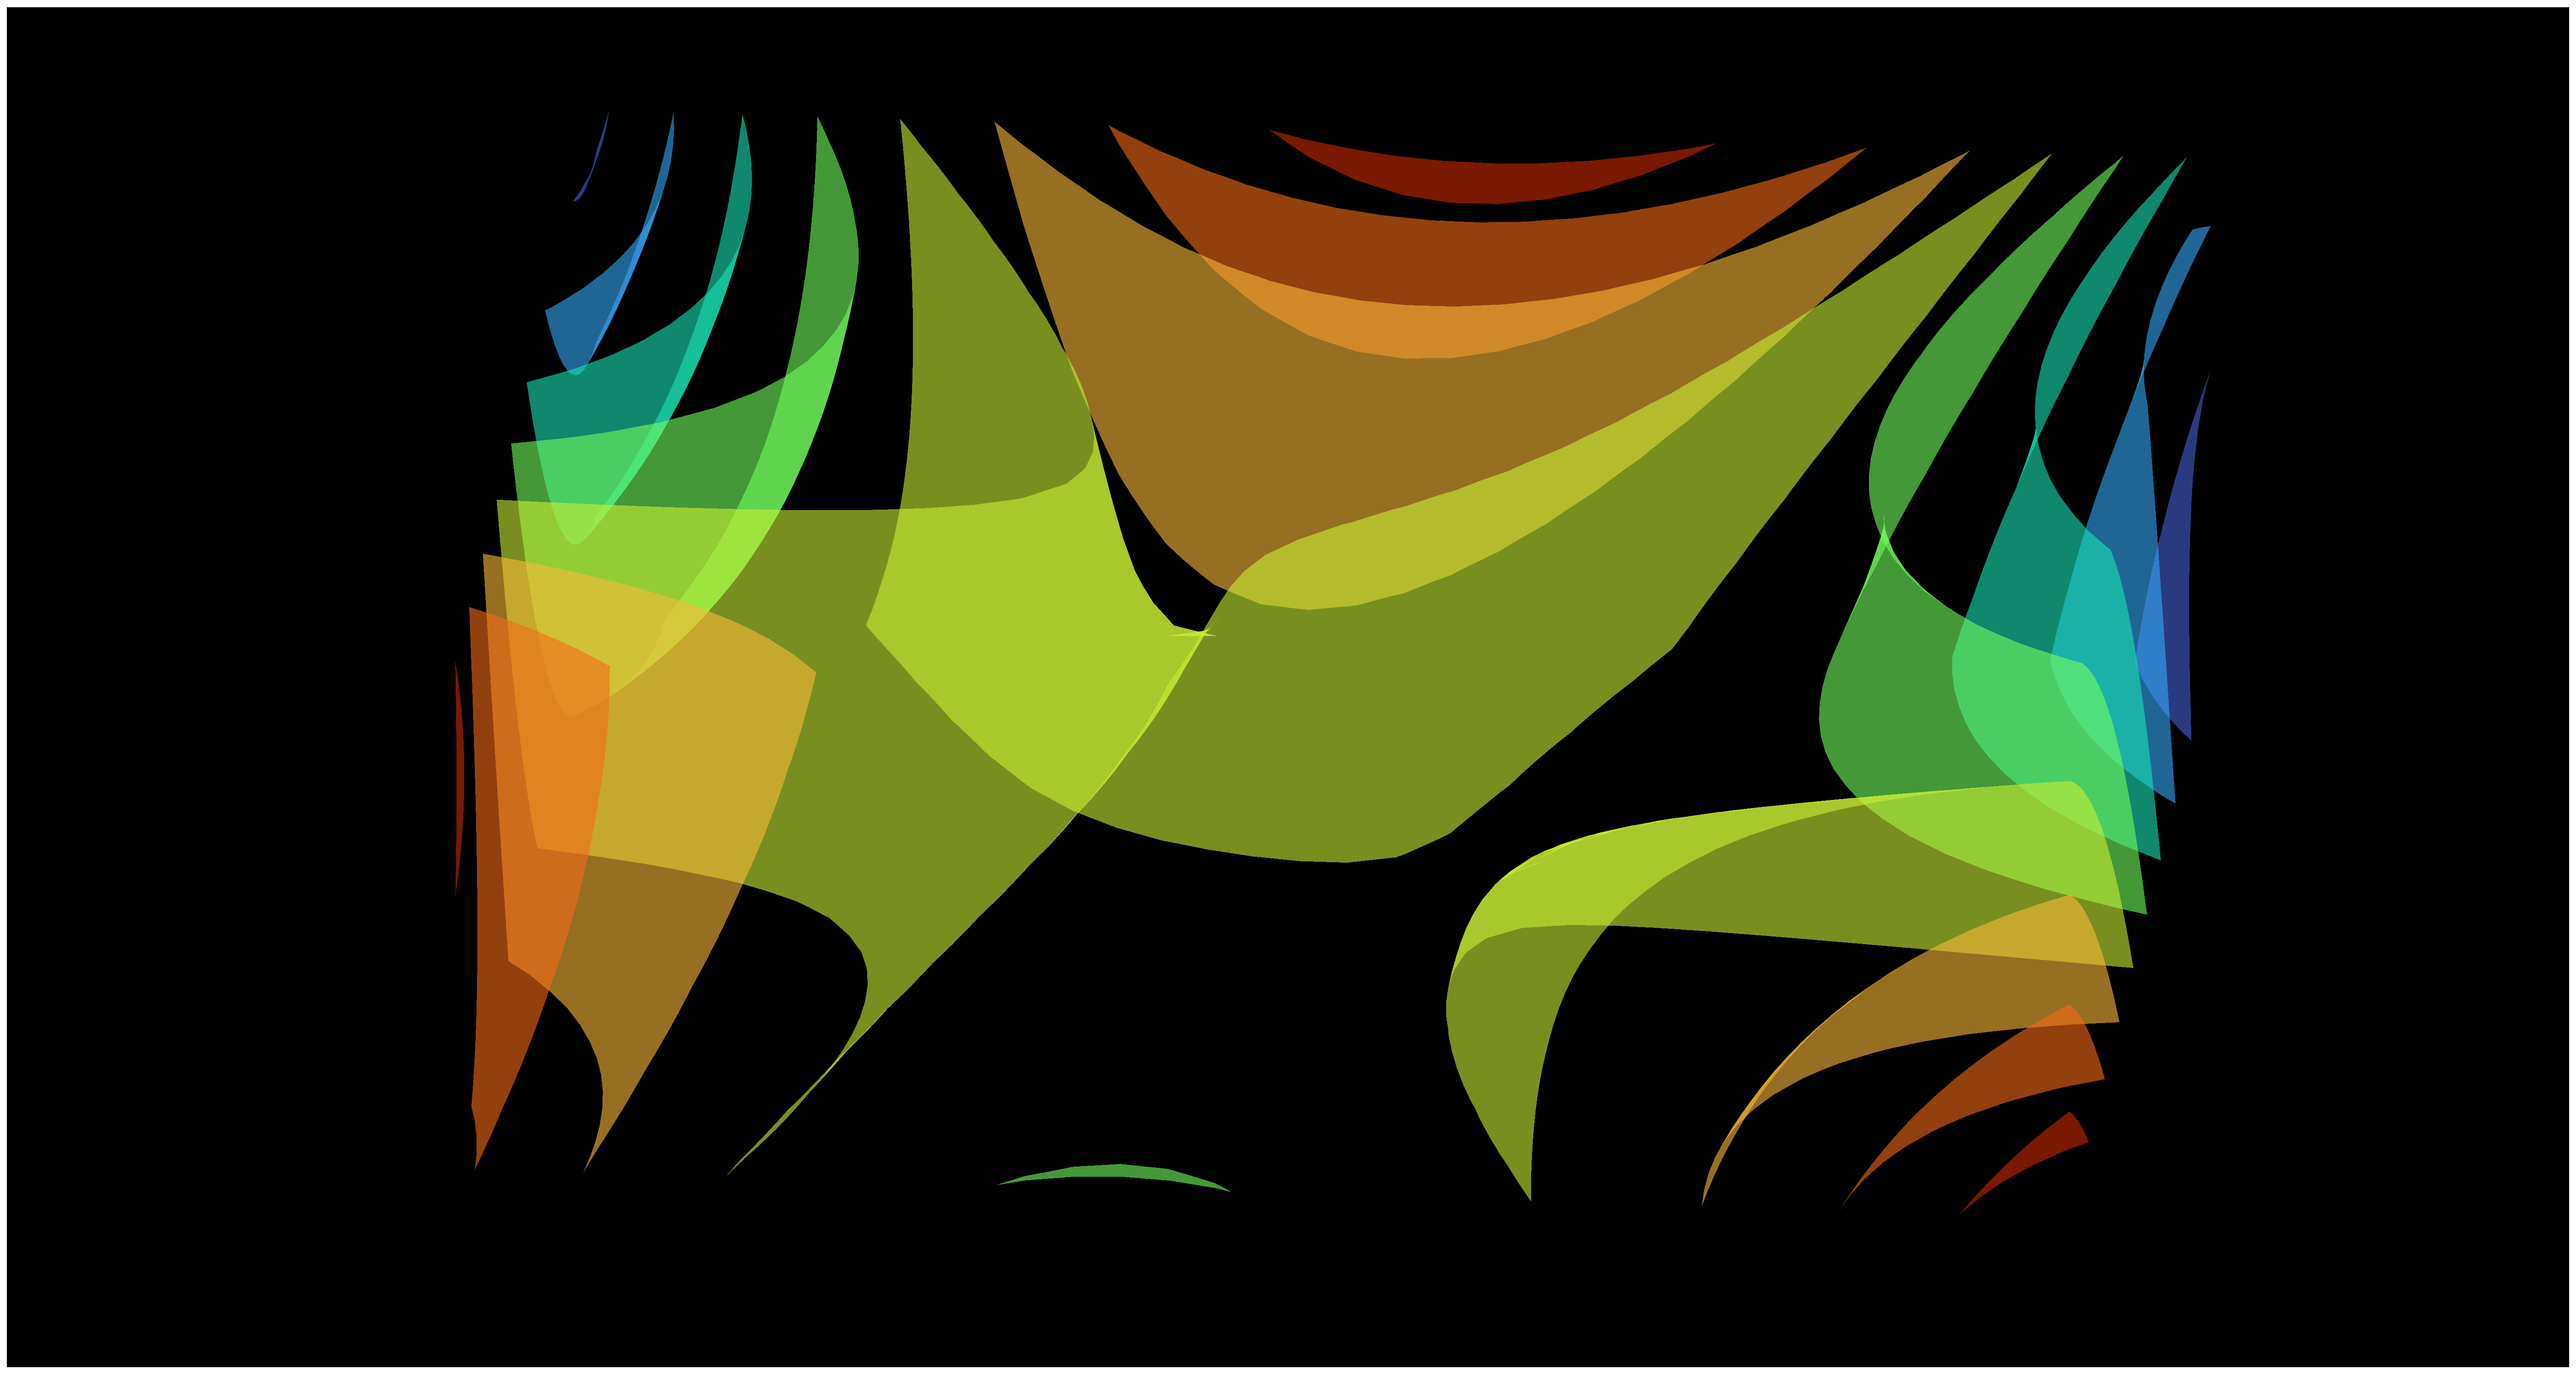
\includegraphics[width=\textwidth]{figures/scalar_field}
\end{figure}
\vfill
\end{frame}

\begin{frame}{Bivector field}
\vfill
The bivector field $A_2 = \proj{2}{}$
\begin{figure}[h]
    \centering
    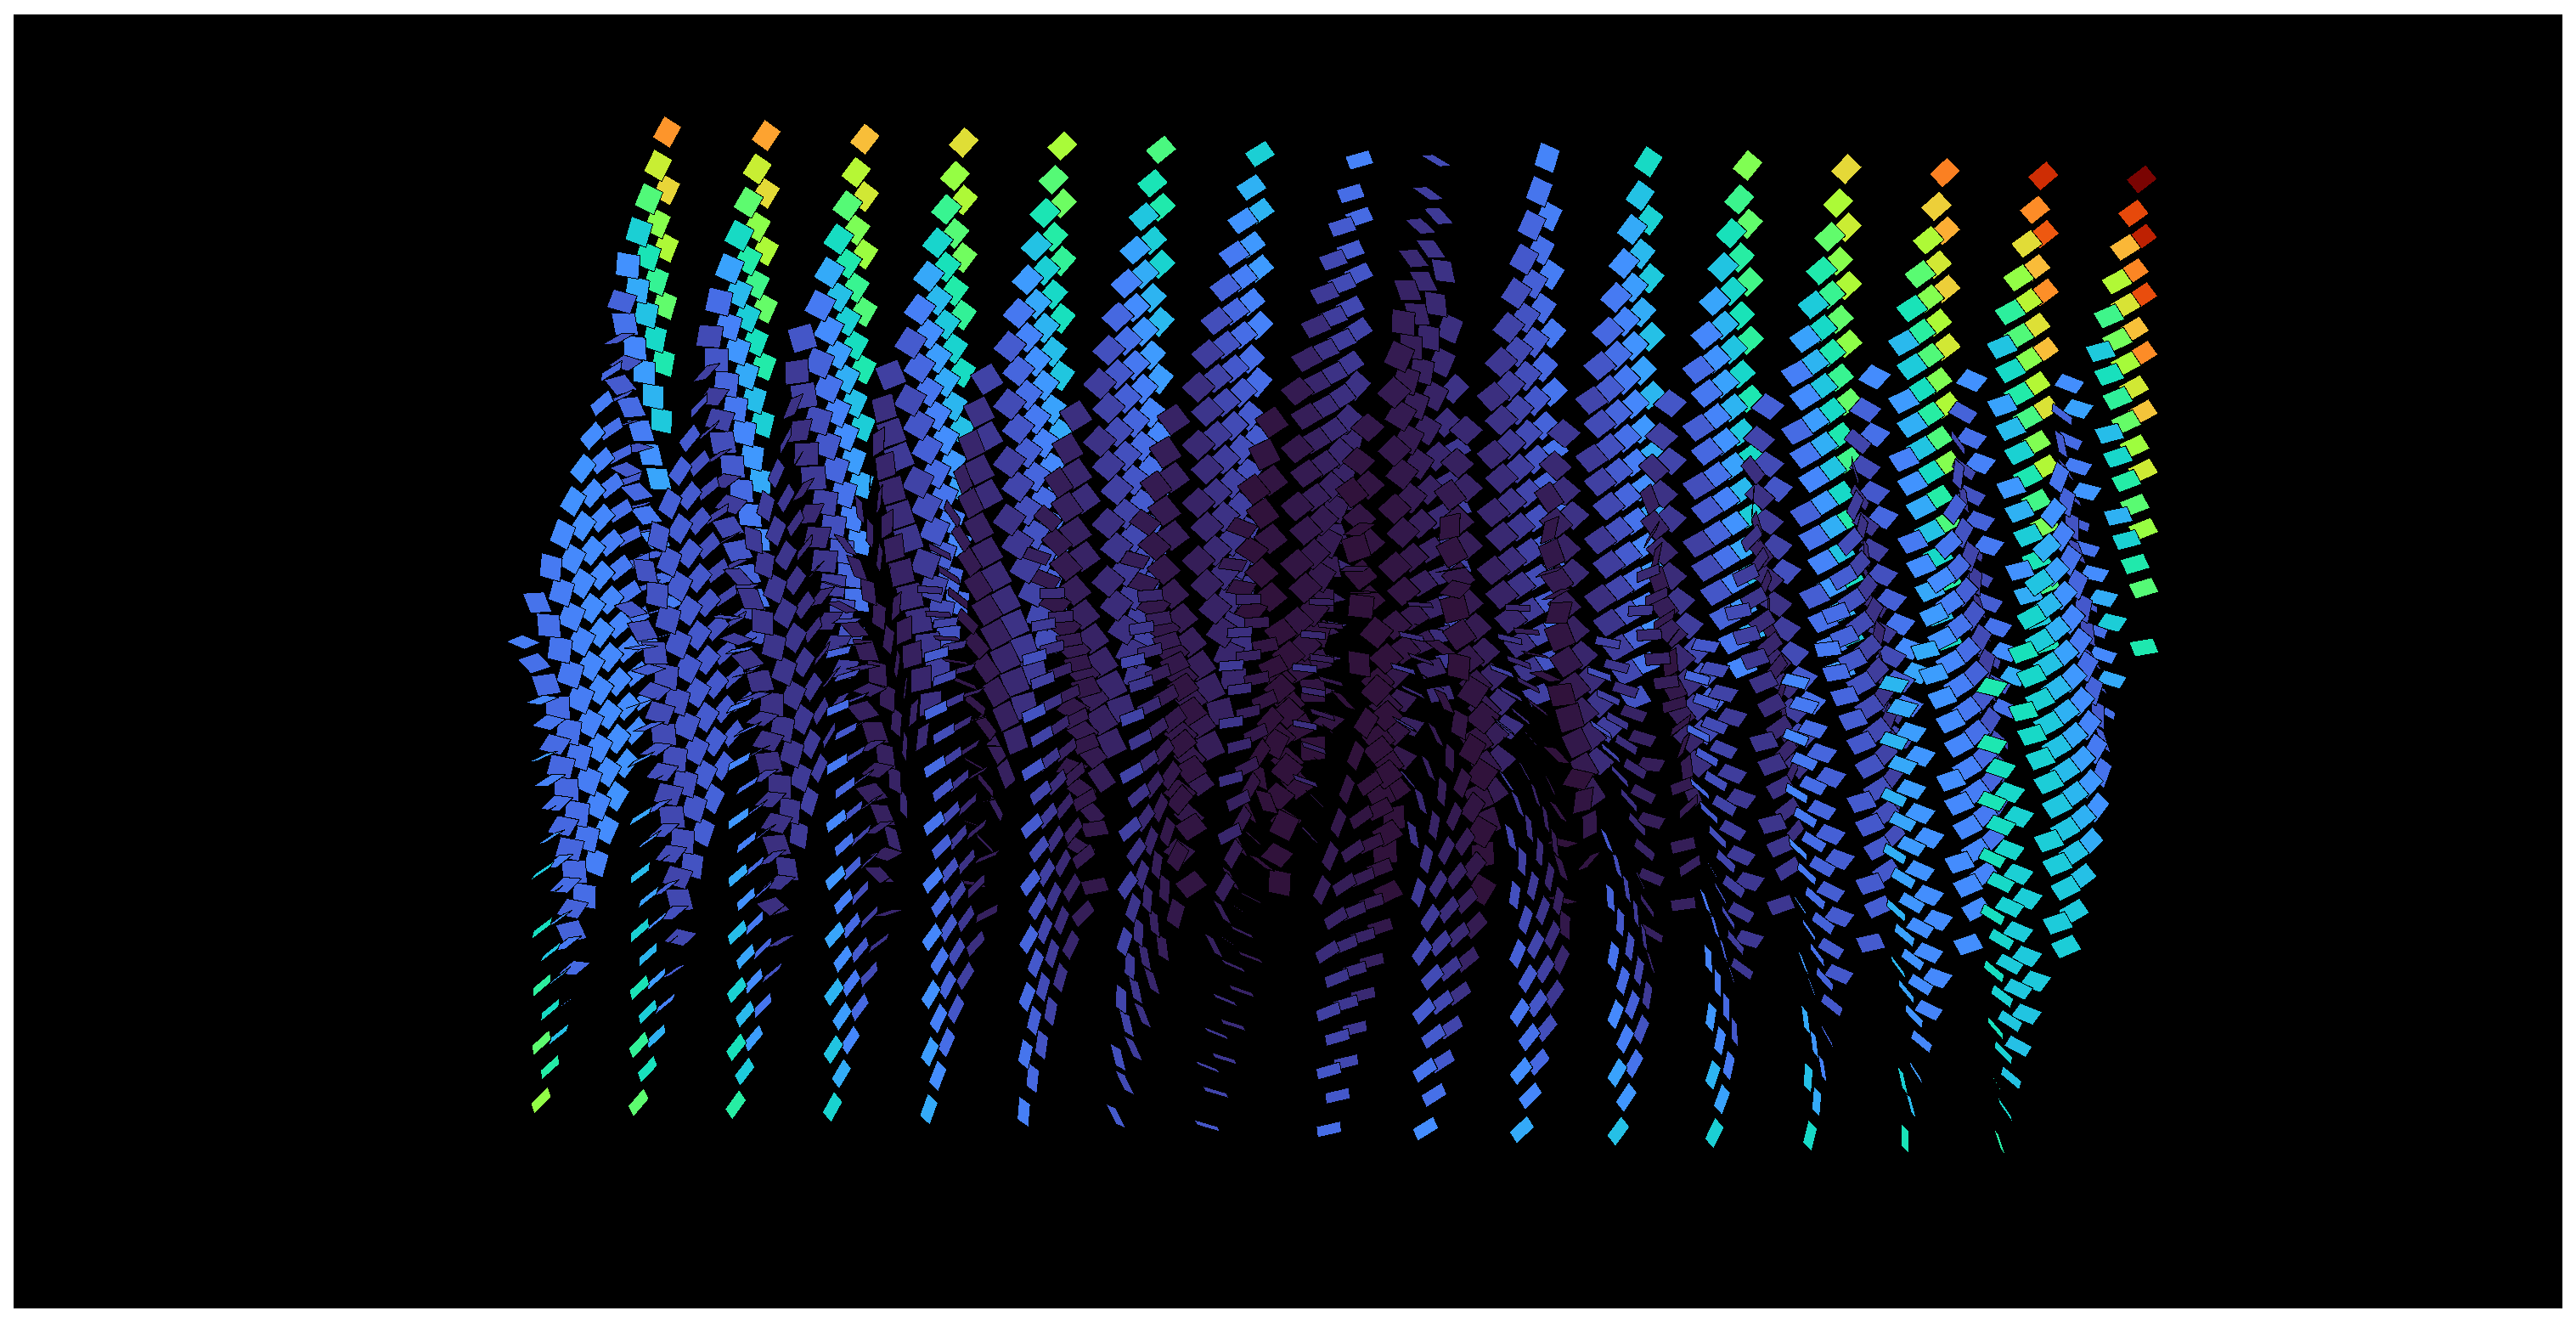
\includegraphics[width=\textwidth]{figures/plane_field}
\end{figure}
\hfill
\vfill
\end{frame}

\begin{frame}{Vector field}
\vfill
The vector field $A_2^\perp$
\begin{figure}[h]
    \centering
    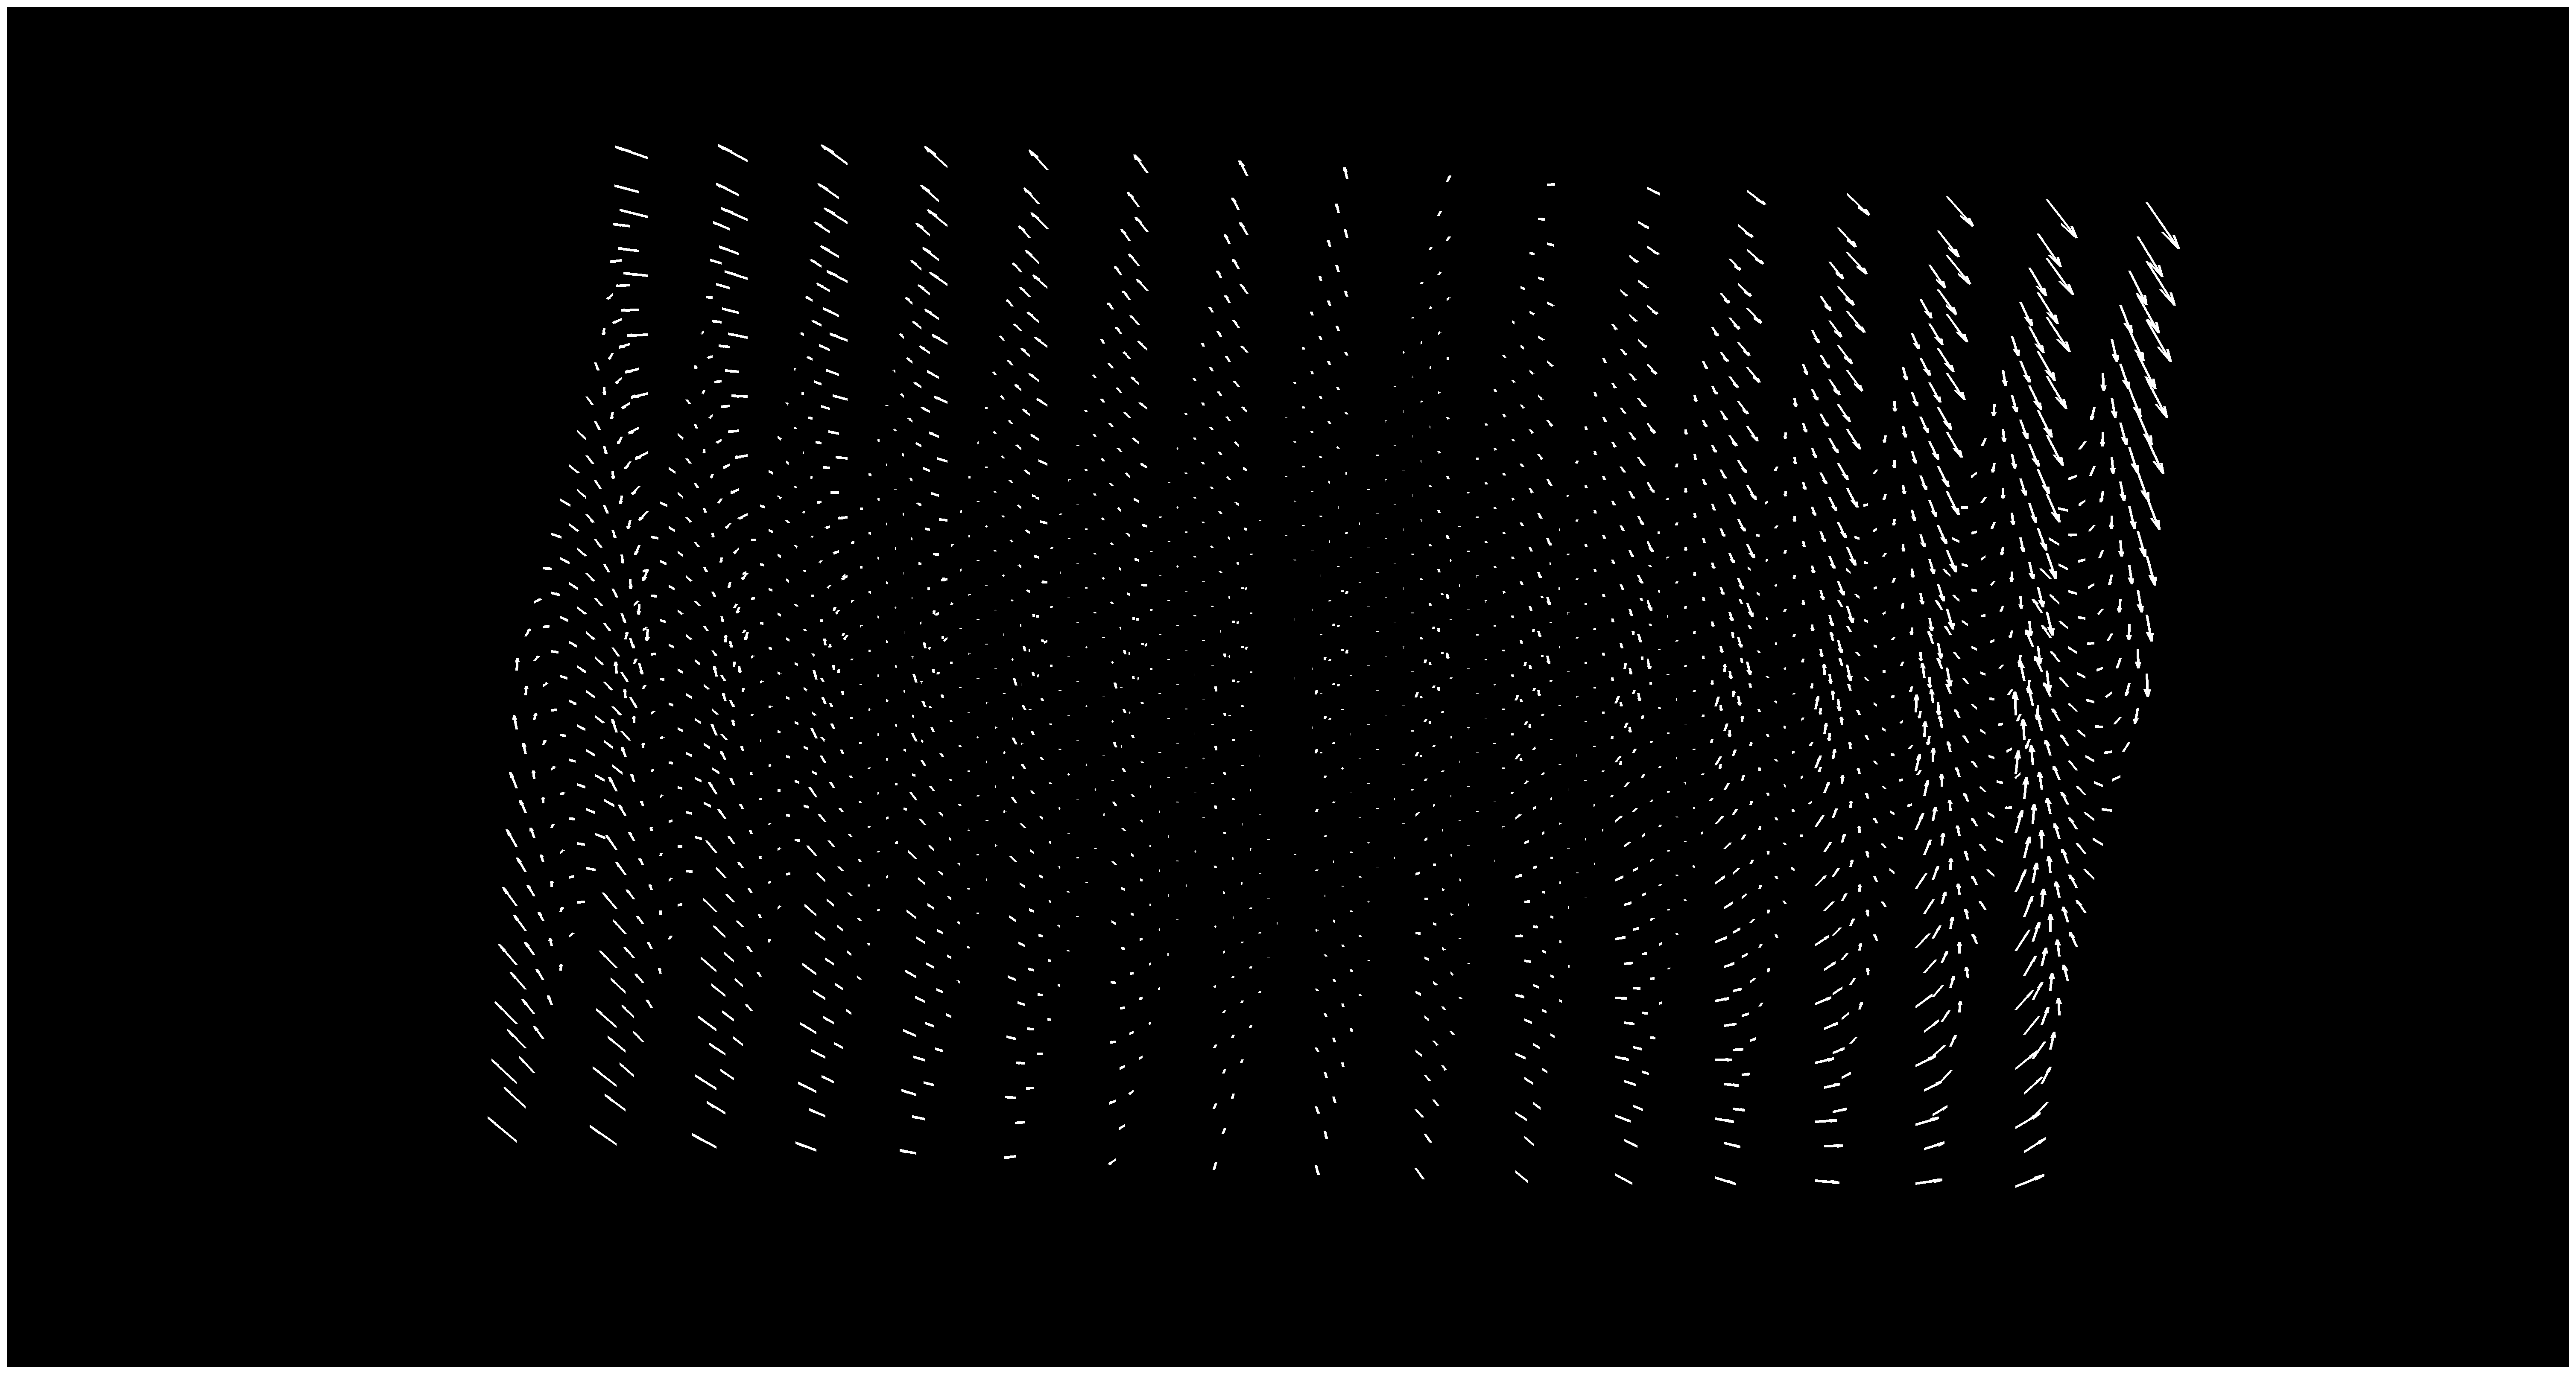
\includegraphics[width=\textwidth]{figures/vector_field}
\end{figure}
\hfill
\vfill
\end{frame}

\begin{frame}{Hodge--Dirac operator}
\vfill
\pause
    $M$ has the Levi-Civita connection $\nabla$ and covariant derivative $\nabla_{\blade{u}}$ which can be extended to act on multivectors \grey{[Schindler: 2018]}.
    \pause
    \begin{itemize}
        \item Define the \boldgreen{Hodge--Dirac operator} locally by
        \[
        \grad = \sum_{i=1}^n \blade{e}^i \nabla_{\blade{e}_i}
        \]
        \pause
        \item $\grad$ acts as a vector in $\smoothfields(M)$ with Leibniz rule $\grad(AB) = \dot{\grad}\dot{A}B + \dot{\grad}A\dot{B}$.
        \pause
        \item $\grad^2$ is the Laplace-Beltrami operator.
    \end{itemize}
\vfill
\end{frame}

\begin{frame}{Examples}
\vfill
\begin{itemize}
\pause
\item For $A_+ \in \smoothfields^+(\R^2)$ if $\grad A_+=0$ then $A_+$ is a \boldgold{holomorphic function}.
\pause
\item For a vector field $\blade{v}\in \smoothfields^1(\R^3)$ we have
    \[
    \grad \blade{v} = \underbrace{\grad \contract \blade{v}}_{\textrm{\boldgold{divergence}}} + \underbrace{\grad \wedge \blade{v}}_{\textrm{\boldgold{curl}}}.
    \]
\pause
\item Specifically,
\[
    \operatorname{curl}(\blade{v}) = (\grad \wedge \blade{v})^\perp
\]
\end{itemize}
\vfill
\end{frame}

\begin{frame}{Differential forms}
\vfill
\begin{itemize}
    \pause
    \item Define the \boldgreen{$r$-dimensional directed measure $dX_r$} by
    \[
    dX_r\coloneqq \blade{e}_{i_1} \wedge \cdots \wedge \blade{e}_{i_r} dx^{i_1} \cdots dx^{i_r}.
    \]
    \pause
    \item Any $r$-form $\alpha_r$ has a \boldgreen{multivector equivalent} $A_r$ so $\alpha_r = A_r \contract dX_r^\dagger$.
    \pause
    \item Algebra and calculus descend to multivector equivalent:
    \begin{align*}
    &\alpha_r \wedge \beta_s = (A_r \wedge B_s) \contract dX_{r+s} & &\alpha_r \contract \beta_s = (A_r \contract B_s) \contract dX_{r-s} \\
  &\underbrace{d\alpha_r = (\grad \wedge A_r) \contract dX_{r+1}^\dagger}_{\textrm{\boldgold{exterior derivative}}} & &\underbrace{\delta \alpha_r = (-\grad \contract A_r) \contract dX_{r-1}^\dagger}_{\textrm{\boldgold{codifferential}}}
    \end{align*}
\end{itemize}
\vfill
\end{frame}

\begin{frame}{Submanifolds}
\vfill
Fix an $r$-dimensional submanifold $R$.
\begin{itemize}
    \pause
    \item Define the \boldgreen{tangent unit pseudoscalar} $\pseudoscalar_R$.
    \pause
    \item Dual is the \boldgreen{normal blade} $\normal_R = \pseudoscalar_R^\perp$.
    \pause
    \item Define the \boldgreen{volume form} on $R$ by
    \[
    d\mu_R \coloneqq \pseudoscalar^{-1}_R \contract dX_r
    \]
    \pause
    \item For $M$ this yields $d\mu = \sqrt{|g|}dx^1\cdots dx^n$
\end{itemize}
\vfill
\end{frame}

\begin{frame}{Integral products}
\vfill
\begin{itemize}
    \pause
    \item Define the \boldgreen{directed integral product on $R$}
    \[
      \directedintproduct{A}{B}_R \coloneqq A^\dagger \pseudoscalar_R B d\mu_R.
    \]
    \pause
    \item Define the \boldgreen{multivector field inner product on $R$} by
    \[
      \multivecinnerproduct{A}{B}_R~ \coloneqq \int_R A \ast Bd\mu_R
    \]
\end{itemize}
\vfill
\end{frame}


\begin{frame}{Green's formulas}
\vfill
\begin{itemize}
    \pause
    \item From \grey{[Hestenes, Sobczyk, 1984]} and \grey{[Boo\ss - Bavnbek, Wojciechowski, 1993]}
    \[
      \directedintproduct{\grad A}{B} = (-1)^n \directedintproduct{A}{\grad B} + \directedintproduct{A}{B}_{\boundary}
    \]
    \pause
    \item Following from the above
    \[
      \multivecinnerproduct{\grad A}{B} = -\multivecinnerproduct{A}{\grad B} + \multivecinnerproduct{A}{\normal B}.
    \]
\end{itemize}
\vfill
\end{frame}

\subsection{Monogenic fields}

\begin{frame}{Monogenic fields}
\vfill
\begin{itemize}
\pause
\item The \boldgreen{monogenic fields $\monogenics(M)$} is the kernel of $\grad$.
\pause
\item Ex. $f=u+v\blade{e}_{12} \in \smoothfields^+(\R^2)$ then $\grad f = 0$ is holomorphic
\begin{align*}
    \frac{\partial u}{\partial x} &= \frac{\partial v}{\partial y}, &
    \frac{\partial u}{\partial y} &= -\frac{\partial v}{\partial x}.
\end{align*}
\end{itemize}
\vfill
\end{frame}

\begin{frame}{}
\makebox[\linewidth]{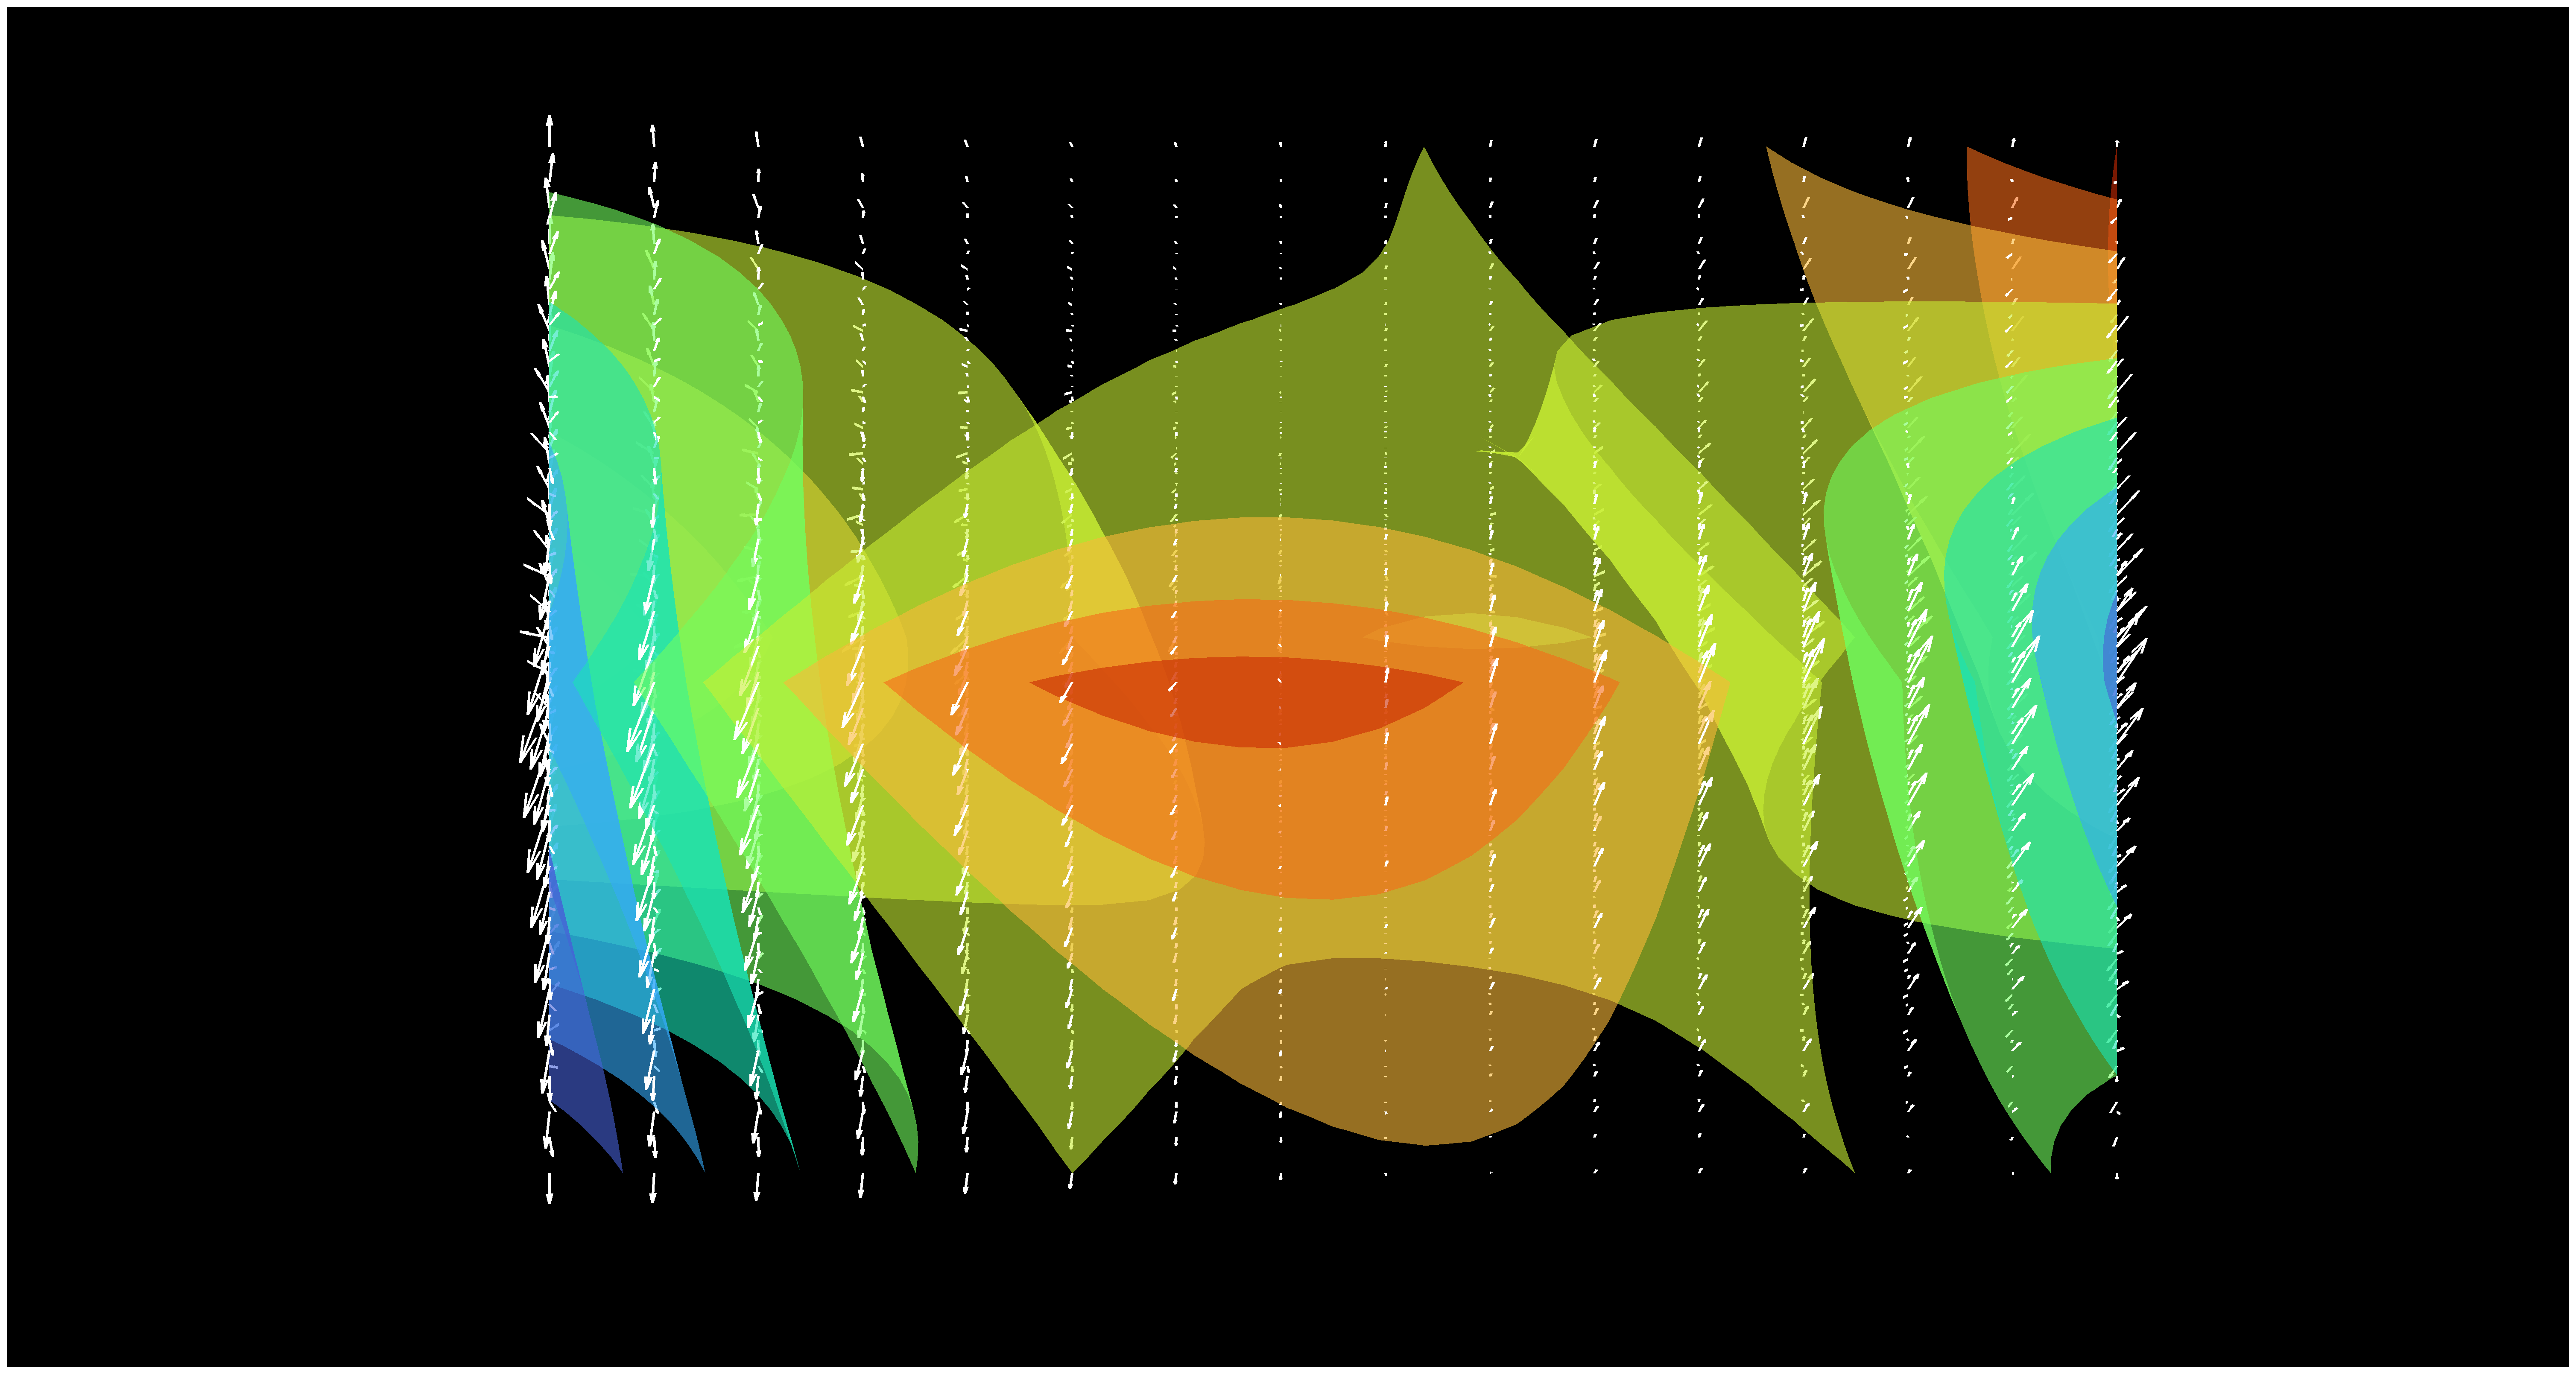
\includegraphics[width=\paperwidth]{figures/monogenic_field}}
% \begin{figure}[H]
%     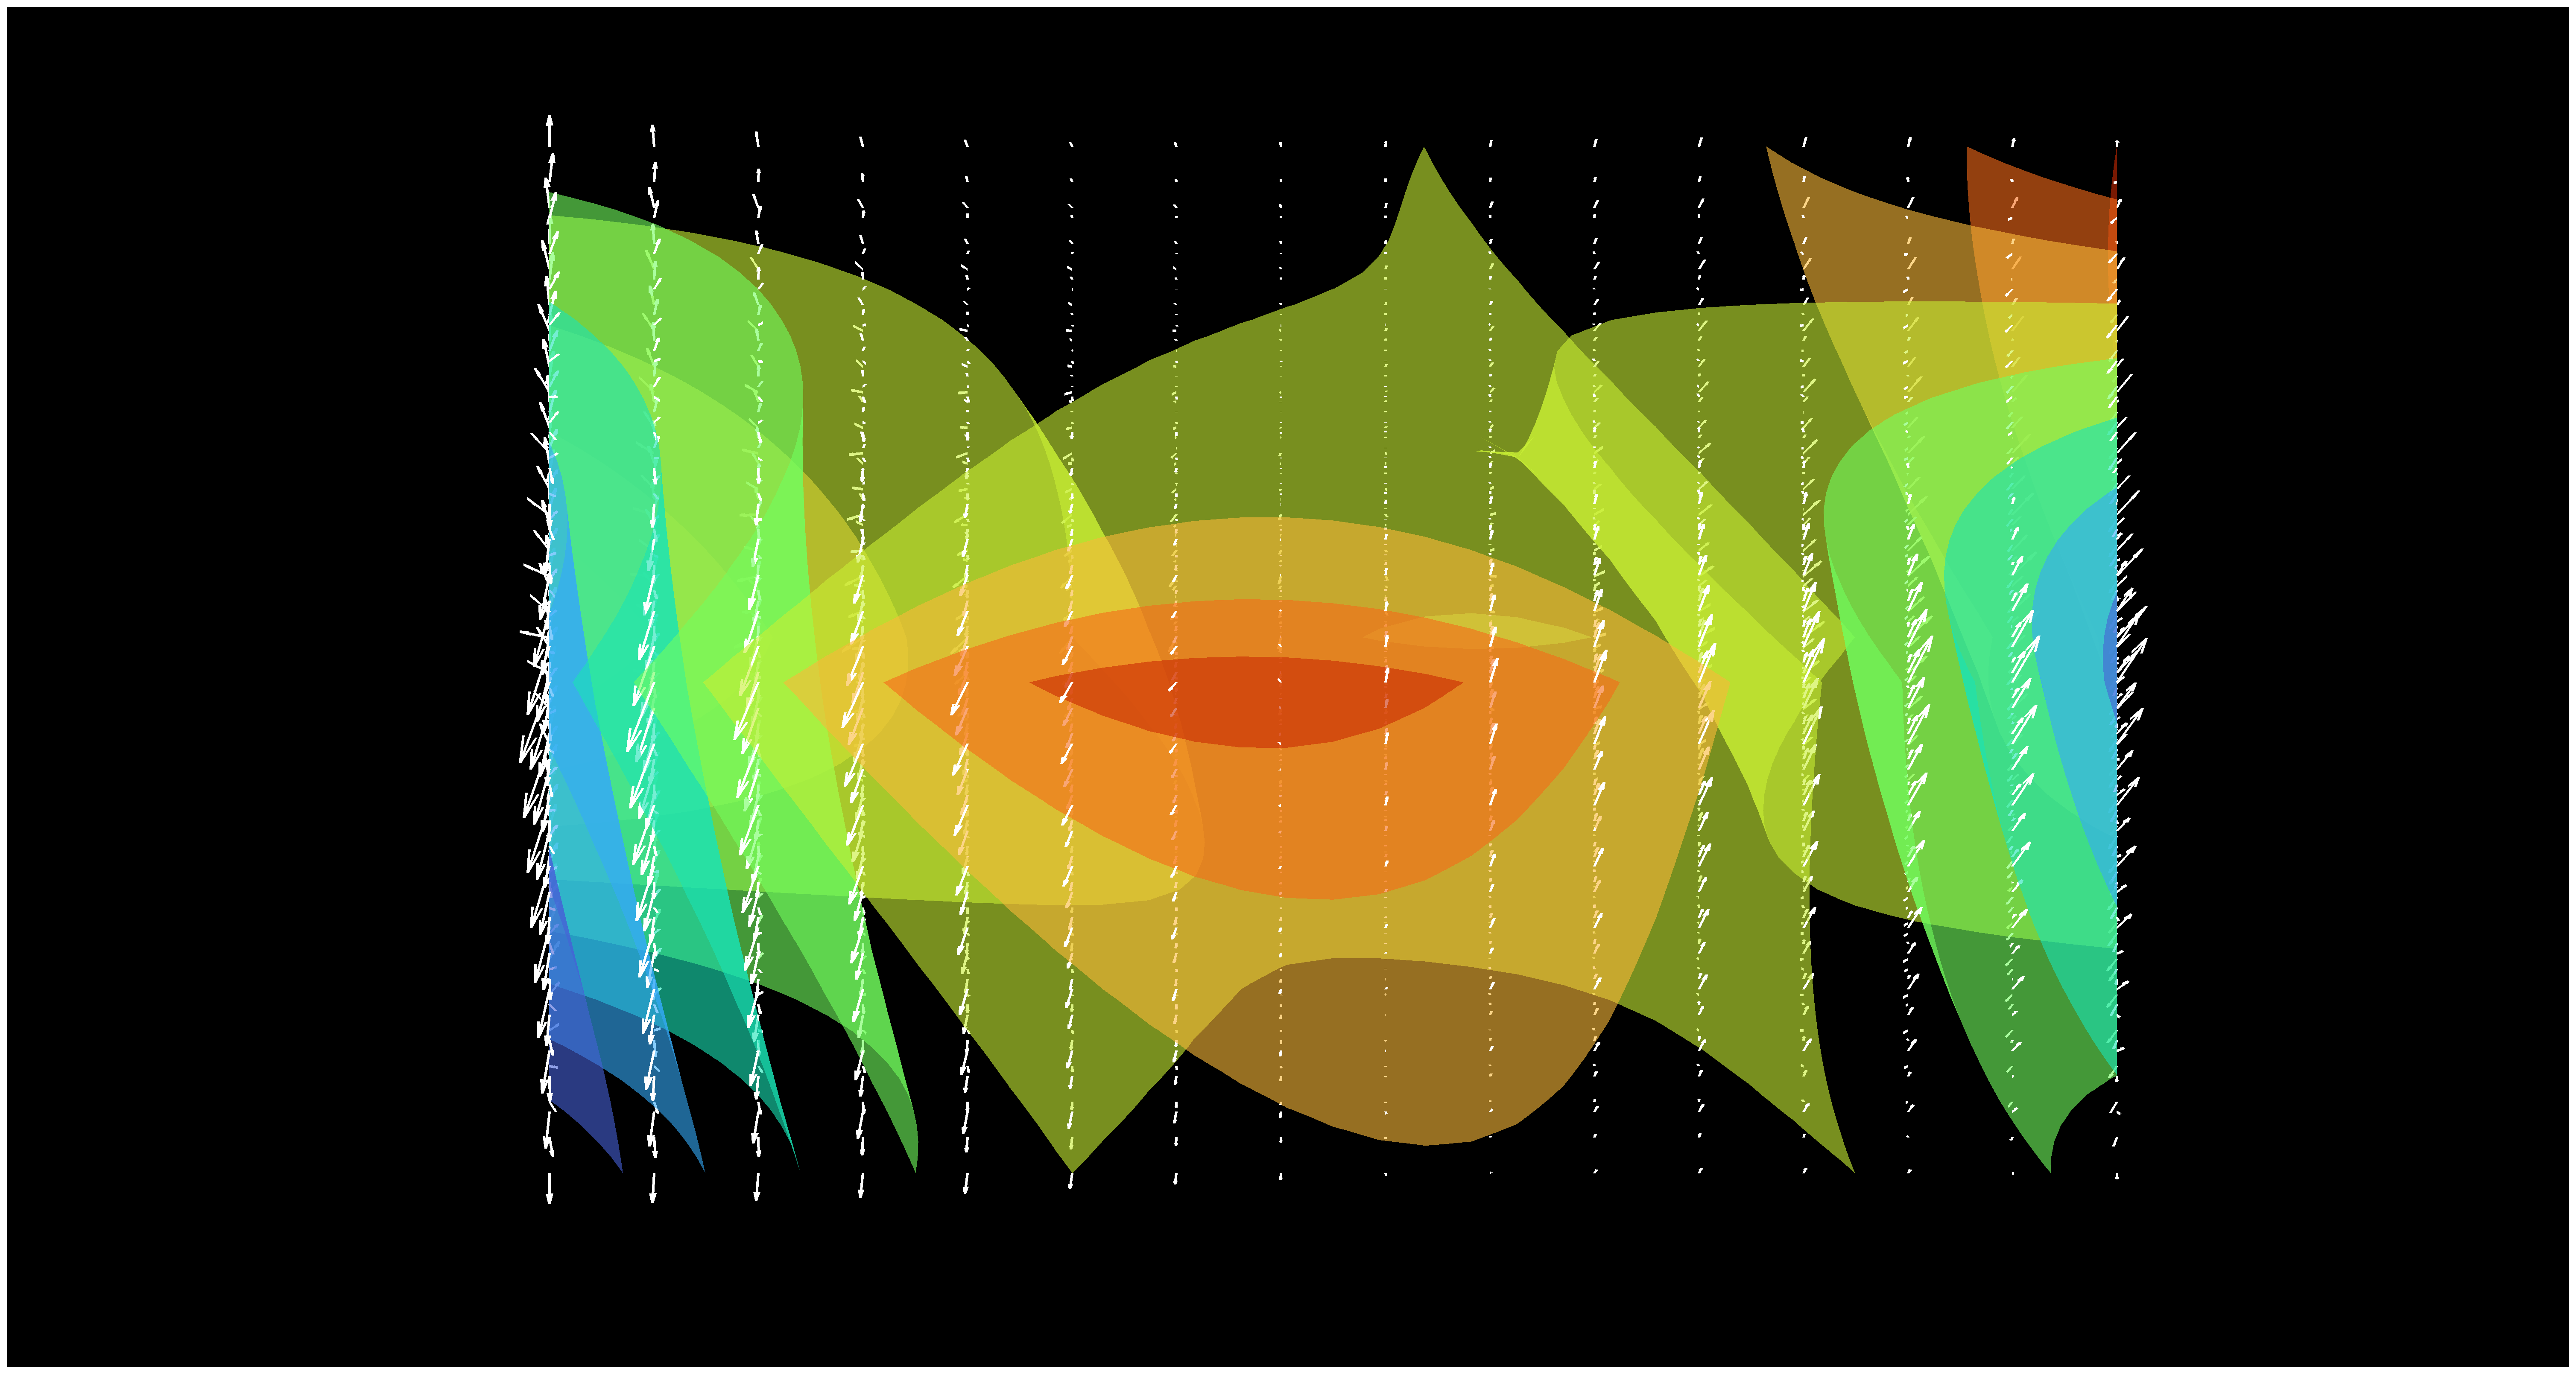
\includegraphics[width=\paperwidth]{figures/monogenic_field}
% \end{figure}
% \hfill
% \vfill
\end{frame}

\begin{frame}{Cauchy integral}
\vfill
There is a map from boundary values $\trace \smoothfields(M)$ to monogenic fields $\monogenics(M)$ \grey{[Calderbank, 1995]}.
\begin{itemize}
\pause
\item There exists a vector-valued \boldgreen{Cauchy kernel} $G_x$ where $\grad G_x = \delta_x$.
\pause
\item Given $A\in \monogenics(M)$, the \boldgreen{Cauchy integral} is
\[
A(x)=(-1)^{n-1}\directedintproduct{A}{G_x}_{\boundary}^\perp.
\]
\end{itemize}
\vfill
\end{frame}

\begin{frame}{Example}
\vfill
Consider fields on a region $M\subset \R^n$:
\begin{itemize}
\pause
\item Define $\blade{G}(\blade{x}) \coloneqq \frac{1}{S_n}\frac{\blade{x}}{|\blade{x}|^n}$ then the Cauchy integral is
\[
A(\blade{x}) = \frac{1}{S_n} \int_\boundary \frac{\blade{x}' - \blade{x}}{|\blade{x}' - \blade{x}|^n}\normal(\blade{x}') A(\blade{x}') d \mu_{\boundary}(\blade{x}').
\]
\pause
\item \boldgold{Scalar part of the above is the double layer potential.}
\end{itemize}
\vfill
\end{frame}

\begin{frame}{Key properties}
\vfill
From \grey{[Calderbank, 1995]}:
\begin{itemize}
\pause
\item \boldgold{Theorem.} $\trace \smoothfields(M) = \trace \monogenics(M) \oplus \normal \trace \monogenics(M)$
\pause
\item Cauchy integral is evaluation and an isomorphism from $\trace \monogenics(M)$.
\vfill
\noindent
\end{itemize}
\end{frame}


\begin{frame}{Inversion}
\vfill
\begin{itemize}
  \pause
  \item \grey{[Calderbank, 1995]} Can solve the equation $\grad A=B$ by
\[
A(x) = (-1)^{n-1}\directedintproduct{B}{G_x}^\perp.
\]
  \pause
  \item In a region $M\subset \R^3$ take a vector field $\blade{J}$,
  \[
  \operatorname{BS}(\blade{J})(\blade{x}) = \proj{2}{\directedintproduct{\blade{J}}{G_{\blade{x}}}^\perp} = \frac{1}{4\pi} \int_{N^3} \blade{J}(\blade{y}) \wedge \frac{\blade{x}'-\blade{x}}{|\blade{x}'-\blade{x}|^{3}} d\mu_{N^3}(\blade{x}').
  \]
  \pause
  \item \boldgold{This is the Biot--Savart formula which recovers magnetic field from current.}
  \end{itemize}
\vfill
\end{frame}

%\begin{frame}{}
%\vfill
%\emph{Proof sketch.}
%\begin{itemize}
%\pause
%\item Use mollifiers to smooth indicator functions $\chi_U$ on open subsets $U$ to be supported only on closed $\epsilon$ neighborhood $\overline{U^\epsilon}$. Call these functions $\chi_U^\epsilon$.
%\pause
%\item Write $A=\sum_J A_J \blade{V}^J$ with $\blade{V}^J = \blade{v}^{j_1}\wedge \cdots\wedge  \blade{v}^{j_r}$. Then note
%    \[
%    \multivecinnerproduct{A}{A_J \blade{V}_J \chi_U^\epsilon} = 0
%    \]
%    implies $A_J=0$ on $U^\epsilon$ for all $J$ since $(\blade{V}^{J}, \blade{V}_K)=\delta^J_K$. Hence $A=0$ on $U^\epsilon$.
%\pause
%\item Cover $M$ in such $U^\epsilon$ and repeat the argument leaving the $A\vert_\boundary$ undetermined. But, by smoothness of $A$, $A=0$ on $\partial M$.
%\end{itemize}
%\vfill
%\end{frame}

\section{Hodge theory}

\begin{frame}{Idea}
\vfill
Hodge theory relates analysis to topology.
\begin{itemize}
  \pause
  \item \boldgold{Theorem (Hodge Isomorphisms).
  \begin{align*}
    H^r(M) &\cong \monogenics^r_N(M) & H^r(M,\boundary)&\cong \monogenics^r(M,\boundary).
  \end{align*}
  }
  \pause
\end{itemize}
\begin{figure}[H]
    \centering
    \def\svgwidth{\columnwidth}
\resizebox{.50\textwidth}{!}{\input{figures/torus_homology.pdf_tex}}
\end{figure}
\vfill
\end{frame}

\begin{frame}{Product on cohomologies}
\vfill
\begin{proposition*}{}{}
The contraction $\contract$ is a product on cohomologies by:
\textcolor{lighter_csu_green}{
\begin{itemize}
\item $\contract \colon H^r(M)\times H^s(M) \to H^{s-r}(M)$;
\item $\contract \colon H^r(M,\boundary)\times H^s(M,\boundary) \to H^{s-r}(M,\boundary)$;
\item $H^r(M)\contract H^s(M,\boundary)$ is trivial;
\item $H^r(M,\boundary)\contract H^s(M)$ is trivial;
\end{itemize}
}
\end{proposition*}
\pause
\begin{itemize}
  \item This product is equivalent to the mixed cup product in \grey{[Shonkwiler, 2009]}.
\end{itemize}
\vfill
\end{frame}


\begin{frame}{Hodge decompositions}
\vfill
Hodge, Morrey, Friedrichs found decompositions of the space of forms.
\begin{itemize}
  \pause
  \item \boldgold{Theorem [Hodge--Morrey]. $\smoothfields^r(M) = \mathcal{E}_D^r(M) \oplus \mathcal{C}_N^r(M) \oplus \monogenics^r(M)$.}
  \pause
  \item \boldgold{Theorem [Hodge--Morrey--Friedrichs].
  \begin{align*}
  \monogenics^r(M) &= \monogenics^r_D(M) \oplus \monogenics^r_{\textrm{co}} &\textrm{or} && \monogenics^r(M) &= \monogenics^r_N(M) \oplus \monogenics^r_{\textrm{ex}}
  \end{align*}
  }
  \pause
  \item \textcolor{red}{But, $\monogenicfields{} \neq \bigoplus_{j=1}^n \monogenicfields{j}$.}
\end{itemize}
\vfill
\end{frame}

\begin{frame}{}
\vfill
The exact and coexact fields satisfy certain boundary constraints. Combining them...
\begin{itemize}
  \pause
  \item Define the \boldgreen{Dirac fields $\grad \smoothfields(M)$} as
  \[
      \grad \smoothfields(M) \coloneqq \{ \grad A ~\vert~ A \in \smoothfields(M) \textrm{~and~} A\vert_\boundary = 0\};
  \]
\end{itemize}
\vfill
\end{frame}


\begin{frame}{}
\vfill
\begin{thm*}{Clifford--Hodge Decomposition}{}
The space of multivector fields $\smoothfields(M)$ has the orthogonal decomposition
\[
\smoothfields(M) = \monogenicfields{} \oplus \grad \smoothfields(M).
\]
\end{thm*}
\vfill
\end{frame}

\begin{frame}{Comparing to Hodge--Morrey}
\vfill
\begin{itemize}
\pause
\item From Hodge--Morrey
\[
\smoothfields(M) = \sum_{r=0}^n \underbrace{\mathcal{E}_D^r(M)}_{\operatorname{Im}(\grad \wedge)} \oplus \underbrace{\mathcal{C}_N^r(M)}_{\operatorname{Im}(\grad \cdot)} \oplus \underbrace{\mathcal{H}^r(M)}_{\operatorname{Ker}(\grad)}.
\]
\pause
\item But the Clifford-Hodge-Morrey is not filtered by grades
\[
\smoothfields(M) = \monogenicfields{} \oplus \grad \smoothfields(M).
\]
\end{itemize}
\vfill
\end{frame}

\section{Tomography}


\begin{frame}{EIT problem}
\vfill
\textcolor{red}{Probably just remove sigma here}
\begin{itemize}
\pause
\item Let $M$ be an Ohmic region of $\R^3$ and $\sigma$ a conductivity.
\pause
\item Ohm's law: $-\sigma \grad\wedge u =\blade{J}$ and conservation $\grad \contract \blade{J}=0$
\pause
\item Suppose $M$ free of charges, then the forward problem
\[
\begin{cases}
\grad \contract (\sigma \grad \wedge u) = 0 & \textrm{in $M$}\\
u = \phi & \textrm{on $\partial M$}
\end{cases}
\]
\pause
\item Define the \boldgreen{electric Dirichlet-to-Neumann (DN) map} $\Lambda_E \colon \tangentpart \smoothfields^0(M) \to \tangentpart \smoothfields^0(M)$ by $\Lambda_E\phi = \normal \contract (\sigma \grad \wedge u)$.
\pause
\item \textbf{\underline{Question:}} Can we determine $(M,\sigma)$ from $\Lambda_E$?
\end{itemize}
\vfill
\end{frame}

\begin{frame}{Magnetic analog}
\vfill
\begin{itemize}
\pause
\item Magnetic bivector field $B$ solves the forward problem
\[
\begin{cases}
\grad^2 B = 0 & \textrm{in $M$}\\
B = \normal \wedge \blade{J} & \textrm{on $\partial M$}
\end{cases}
\]
\pause
\item Define the \boldgreen{magnetic DN operator} $\Lambda_B \colon \normalpart \smoothfields^2(M) \to \normalpart \smoothfields^2(M)$ by $\Lambda_B(\normal \wedge \blade{J}) = \normal \wedge \grad \contract B$.
\pause
\item \textbf{\underline{Question:}} What can we get from $\Lambda_B$?
\end{itemize}
\vfill
\end{frame}

\begin{frame}{Electromagnetic tomography}
\vfill
\begin{itemize}
\pause
\item \boldgold{Can combine to monogenic spinor $A_+=u+B$.}
\pause
\item Can we recover the space of monogenic fields from the DN operators?
\pause
\item If the space of monogenic fields contained geometric data, this would be a step forward in the Calder\'on problem...
\end{itemize}
\vfill
\end{frame}

\begin{frame}{Calder\'on problem}
\vfill
Don't forget our goal...
\begin{itemize}
\pause
    \item The problem has been solved in dimension $n=2$ \grey{[Belishev: 2003]}.
\pause
    \item Solved in dimensions $n\geq 3$ when $M$ is an analytic manifold \grey{[Lassas, Taylor, Uhlmann: 2003]}.
\pause
\item The smooth cases is still unsolved.
\end{itemize}
\vfill
\end{frame}


\begin{frame}{Geometric generalization}
\vfill
\begin{itemize}
\pause
\item Allow $M$ to be $n$-dimensional manifold.
\pause
\item Use intrinsic metric $g$ and forward problem for $r$-vector fields
\[
\begin{cases}
\grad^2 A_r = 0 & \textrm{in $M$}\\
A_r = \phi_r & \textrm{on $\partial M$}
\end{cases}
\]
\pause
\item \boldgreen{Generalized electric DN operator} by $\Lambda_E \colon \tangentpart \smoothfields(M) \to \tangentpart \smoothfields(M)$ by $\Lambda_E \phi_r = \normal \contract \grad \wedge A_r$.
\pause
\item \boldgreen{Generalized magnetic DN operator} by $\Lambda_B \colon \normalpart \smoothfields(M) \to \normalpart \smoothfields(M)$ by $\Lambda_B \phi_r = \normal \wedge \grad \contract A_r$.
\end{itemize}
\vfill
\end{frame}


\begin{frame}{Comologies from DN operators}
\vfill
\begin{itemize}
\pause
\item The kernel of $\Lambda_E$ are tangent parts of $\monogenics_N^r(M)$.
\pause
\item The kernel of $\Lambda_B$ are normal parts of $\monogenics_D^r(M)$.
\pause
\item These components uniquely determine elements of $\monogenics_N^r(M)$ and $\monogenics_D^r(M)$ respectively.
\pause
\item Applying Hodge isomorphisms...
\end{itemize}
\begin{thm*}{}{}
We have $\ker \Lambda_E \cong H^r(M)$ and $\ker \Lambda_B \cong H^r(M,\boundary)$.
\end{thm*}
\begin{itemize}
  \item The map $\Lambda_E \times \Lambda_B$ is equivalent to \boldgold{complete DN operator $\Pi$} \grey{[Shonkwiler, Sharafutdinov: 2013]}.
\end{itemize}
\vfill
\end{frame}

\begin{frame}{Spinor DN operator}
\vfill
\begin{itemize}
\pause
\item Define the \boldgreen{spinor DN operator} $\mathcal{J}\colon \trace \smoothfields^\pm(M) \to \trace \smoothfields^\pm(M)$.
\pause
\item Specifically: $\mathcal{J}\phi_r = \normal \grad A_r$.
\pause
\item Generalized operators are scalar part $\Lambda_E+\Lambda_B = \proj{}{\mathcal{J}}$.
\end{itemize}
\pause
\begin{thm*}{}{}
We have $\ker \mathcal{J} = \trace \monogenics(M)$.
\end{thm*}
\begin{itemize}
  \item \boldgold{Recall $\trace \monogenics(M)$ in correspondence to $\monogenics(M)$ by Cauchy integral.}
\end{itemize}
\vfill
\end{frame}

\section{Gelfand theory}

\begin{frame}{Open questions}
\vfill
\begin{itemize}
\pause
    \item In \grey{[Belishev: 2003]}, we see an algebraic proof for the 2-dimensional Calder\'on problem.
\pause
    \item In \grey{[Belishev, Vakulenko: 2017]}, we see a proof for a noncommutative Gelfand representation using quaternion fields for a ball $\ball$ in $\R^3$.
\pause
    \item Belishev and Vakulenko as whether this is true in higher dimensions.
\pause
    \item We will prove this is true for arbitrary regions.
\end{itemize}
\vfill
\end{frame}

\begin{frame}{Overview of BC method}
\vfill
The \boldgreen{boundary control (BC) method} in \grey{[Belishev: 2003]} is as follows:
\begin{itemize}
    \pause
    \item Determine the algebra $\algebra{}(M)$ of holomorphic functions on $M$ using $\Lambda$.
    \pause
    \item Gelfand theory implies the spectrum of $\algebra{}(M)$ is homeomorphic to $M$.
    \pause
    \item Algebraic structure of $\algebra{}(M)$ determines the complex structure on $M$.
    \pause
    \item Find $g$ that conformal with the complex structure.
\end{itemize}
\vfill
\end{frame}

\begin{frame}{Subsurface spinor fields}
\vfill
\begin{itemize}
\pause
\item For $O$ convex, let $\bivector \in \smoothfields(O)$ be parallel translation of a unit $2$-blade.
\pause
\item Refer to $A_+ = \projection_{\bivector} \circ A_+$ as a \boldgreen{subsurface spinor}.
\pause
\item The \boldgreen{algebra of monogenic subsurface spinors} is $\algebra_{\bivector}(O)$
\pause
\item \boldgold{Algebra is a commutative Banach algebra (isomorphic to holomorphic functions).}
\end{itemize}
\begin{figure}[H]
    \centering
    \def\svgwidth{\columnwidth}
\resizebox{.4\textwidth}{!}{\input{figures/foliation.pdf_tex}}
\end{figure}
\vfill
\end{frame}


\begin{frame}{$z$ analogs and polynomials}
\vfill
\begin{itemize}
\pause
\item Define the functions $z_{ij}=x_j-x_i \blade{e}_{ij}$.
\pause
\item Then $z_{ij} \in \algebra_{\blade{e}_{ij}}(O)$.
\pause
\item A \boldgreen{homogeneous monogenic polynomial} is
\[
p_{\vec{k}} = \frac{1}{k!} \sum_{\sigma} z_{1\sigma(1)}\cdots z_{1\sigma(k)}.
\]
\pause
\item Space of \boldgreen{monogenic polynomials} is $\mathrm{span}_\G \{p_{\vec{k}}\}$.
\end{itemize}
\vfill
\end{frame}

\begin{frame}{}
Locally on $M$ any monogenic field can be written as a power series.
\end{frame}

\begin{frame}{Idea}
\vfill
\begin{itemize}
\pause
\item By linearity, we can note that for $\delta \in \characters(\ball_{R,w})$
\[
\delta(f(x)) = \sum_{j=0}^\infty \left(\sum_{\substack{{j_2 \cdots j_n} \\ {j_2 + \cdots + j_n = j}}} \delta(p_{j_2 \cdots j_n} (x-w)) a_{j_2 \cdots j_n} \right)
\]
\pause
\item On each monogenic polynomial
\[
\delta(p_{j_2 \dots j_n}(x)) = \frac{1}{j!} \sum_{\textrm{permutations}}\delta\left((z_{1\sigma(1)}(x)\right) \cdots \delta\left(z_{1\sigma(j)}(x)\right)
\]
by the multiplicativity of $\delta$.
\end{itemize}
\vfill
\end{frame}

% \begin{frame}{Functionals}
% \vfill
% \begin{itemize}
% \pause
% \item Define the \boldgreen{spinor dual} $\dualmonogenics(M)$ as the continuous right $\G_n^+$-module homomorphisms
% \[
% \dualmonogenics(M) \coloneqq \{ l \colon \monogenicfields{+} \to \G_n^+ ~\vert~ l(fs+g)=l(f)s+l(g), ~\forall f,g\in \monogenicfields{}, ~s \in \G_n^+\}
% \]
% and refer to the elements as \boldgreen{spin functionals}.
% \pause
% \item Assert the weak-$\ast$ topology on $\dualmonogenics(M)$ so that every $x\in M$ corresponds to a continuous map on $\monogenics^+(M)$.
% \end{itemize}
% \vfill
% \end{frame}



\begin{frame}{Characters}
\vfill
\begin{itemize}
\pause
\item Define the algebra $\mathbb{A}_{\bivector}$ to be the algebra generated by $1$ and $\bivector$.
\pause
\item The \boldgreen{spinor spectrum} $\characters(M)$ consists of \boldgreen{spin characters}:
\begin{itemize}
  \item Continuous grade-preserving $\G^+$-linear maps $\monogenics^+(M) \to \G^+$,
  \item algebra morphisms $\algebra_{\bivector}(O) \to \mathbb{A}_{\bivector}$.
\end{itemize}
\pause
\item One example of such characters are point evaluations $\delta(A_+)=A_+(x_\delta)$.
\pause
\item We show these are the only elements in the spectrum.
\end{itemize}
\vfill
\end{frame}


\begin{frame}{Necessary lemmas}
\vfill
\pause
For regions $M\subset \R^n$:
\pause
\begin{lemm*}{Density}{}
The space $\monogenics^\mathcal{P}(M)$ is dense in $\monogenics(M)$.
\end{lemm*}
\pause
\begin{lemm*}{Point evaluation}{}
For $\delta \in \characters(M)$ we have $\delta(z_{ij})=z_{ij}(x_\delta)$ for some $x_\delta \in \R^n$.
\end{lemm*}
\pause
\begin{lemm*}{Identification}{}
Let $A_+\in \mathcal{M}^+(M)$, then $\delta (A_+)=A_+(x_\delta)$ for some $x_\delta \in M$.
\end{lemm*}
\vfill
\end{frame}

\begin{frame}{}
\vfill
The previous lemmas imply the following:
\pause
\begin{thm*}{Clifford-algebraic Gelfand theorem}{}
With the weak-$\ast$ topology on $\characters(M)$, the map
\[
\gamma \colon \characters(M) \to M, \quad \delta \mapsto x_\delta
\]
is a homeomorphism. The Gelfand transform $\widehat{A_+}(\delta)=\delta[A_+]$ is an isometric isomorphism so $\monogenics^+(M) \cong \widehat{\monogenics^+(M)}$.
\end{thm*}
\vfill
\end{frame}




\section{Further results, open questions, conclusion}
%
  \begin{frame}{A Stone--Weierstrass theorem}{}
\vfill
\begin{lemm*}
If $M$ is a compact connected Riemannian manifold with boundary, then the space $\overline{\monogenics^+(M)}$ separates points.
\end{lemm*}

\begin{thm*}{Stone--Weierstrass}{}
$\vee \overline{\monogenics^+(M)}$ is dense in $C(M;\G^+)$.
\end{thm*}
\vfill
\end{frame}

\begin{frame}{Sheaf}
\vfill
\begin{thm*}{}{}
The sheaf $\monogenics_M$ is Hausdorff and the map $\pi \colon \monogenics_M \to M$ is a local homeomorphism.
\end{thm*}
\begin{itemize}
  \item Can one find a component of $\monogenics_M$ that is homeomorphic to $M$?
\end{itemize}
\vfill
\end{frame}


\begin{frame}{Future work and open questions}
\vfill
To get a higher dimensional BC method we need:
\begin{itemize}
  \item The DN operator determines $\trace \monogenics^+(M)$.
  \item The map $\trace \colon \vee \monogenics^+(M) \to \trace \vee \monogenics^+(M)$ is an isometric isomorphism of algebras.
  \item The space $\monogenics^+(M)$ determines the metric structure of $M$ up to isometry.
\end{itemize}
\vfill
\end{frame}


\begin{frame}{Future work and open questions}
\vfill
\begin{itemize}
  \item Many of these approaches use the Hilbert transform which is also used by Belishev, Sharafutdinov, and Shonkwiler to study the Calder\'on problem.
  \item The Hilbert transform is also a classical part of Clifford analysis.
  \item \grey{[Lassas, Uhlmann: 2001]} use sheaf theory to solve the analytic Calder\'on problem.
  \item Santacesaria proposes another method for solving the Calder\'on problem using Clifford algebras and complex geometric optics.
\end{itemize}
\vfill
\end{frame}

\section{Conclusions}

\begin{frame}{Conclusion}
\vfill
\begin{itemize}
\pause
    \item Clifford analysis is a natural setting for studying PDEs and Hodge theory on manifolds.
\pause
    \item Able to describe DN operators and extract homological information and boundary values of special functions.
\pause
    \item Special functions are able to tell us the topology of the manifold they are defined on.
\end{itemize}
\vfill
\end{frame}


\begin{frame}{}
\vfill
\begin{center}
\large Thank you!
\end{center}
\vfill
\end{frame}

\end{document}
